\chapter{Track Finding in basf2} \label{chapter-workflow}

After having described the principle of the track finders implemented in basf2 in the previous chapters, the actual changes to the software implementation during this thesis are discussed in this chapter. Before going into detail, the figures of merit of the two track finders showing their advantages and drawbacks are presented in the first section. After a short introduction in the general structure, the newly implemented background hit finder and the performed improvements on the stereo Legendre track finder are shown. Then the newly written \texttt{SegmentTrackCombinerDevModule} is described. The chapter ends with a section on general tools how to improve the found track candidates and an outlook.

All the plots showing recent results are done with the svn revision 21844. If the implementation before this thesis is compared to the recent results, svn revision number 18262 is used.

\section{FOM of the two track finders} \label{section-fom}

In the following, the figures of merit of the both track finders -- the local and the global one -- are shown as they were before the works during this thesis. For comparison, the reference implementation trasan is shown. Trasan is the old track finder algorithm developed for the former Belle detector and was adopted to the new Belle~II geometry. It was highly optimized in the run of the experiment but will not be used for the Belle~II experiment, as it is neither build on modern programming principles nor easy to extend by other algorithms and most of the time also poorly documented. However, the figures of merit of trasan are the leveling staff every new track finder has to be compared with as also done in the following.

Table~\ref{tab-old-implementation-results} shows the overall figures of merit for the two track finders running standalone together with trasan. A detailed analysis can be found below. The table shows the finding and hit efficiency together with the clone and fake rate as described in chapter~\ref{chapter-theory} aggregated over 1000 generic $\PB \APB$-events simulated with background hits. Together with these figures of merit, also the numbers for primaries only are calculated using the \verb+isPrimary+ flag of the MC particles. As therefore a correct matching between tracks from the track finders and the MC particles is needed, it can only be calculated for non-fake tracks. This is why the fake rate for primaries only is meaningless and not shown in the table. The time per event is measured with the basf2-own performance tools and are machine-dependent. All figures presented in this thesis were calculated using the same desktop machine.

As expected because of the high degree of optimization of trasan, both the Legendre and the automaton track finder can not reach the figures of merit of the reference implementation. Additionally, the Legendre track finder is much slower than trasan which is mainly due to a non-optimized stereo hit finder that will be discussed in section~\ref{section-stereo}. The automaton track finder has the worst figures of merit when it comes to efficiency. The problems in the implementation lay in the combination of the found segments in the second step (refer to chapter~\ref{chapter-theory}), which fails in most of the cases. As can be seen below the purity and efficiency is very high when using the segments alone.

\begin{table}
  \caption{Table showing the figures of merit for the two track finder implementations (global and local) and trasan.}
  \centering
  \begin{tabular}{lccc} \toprule
    & Legendre & Automaton & Trasan \\ 
    & \multicolumn{2}{c}{Track Finder} & \\ \midrule
    Finding Efficiency & 83.17 & 12.84 & 85.53 \\
    \quad on Primaries & 89.94 & 14.20 & 91.49 \\ 
    Hit Efficiency     & 74.03 & 58.29 & 81.93 \\
    \quad on Primaries & 78.22 & 59.76 & 87.25 \\ 
    Clone Rate         & 7.69  & 14.02 & 19.50 \\
    \quad on Primaries & 4.71  & 26.54 & 17.17 \\ 
    Fake Rate          & 26.82 & 48.17 & 15.95 \\ 
    Time per Event in ms & 635.05 & 31.92 & 419.50 \\ \bottomrule
  \end{tabular}
  \label{tab-old-implementation-results}
  % Using InputData 2
  % Trasan should show the same numbers. Legendre should be the same as in Stereo. Automaton is irrelevant, as never used like this.
  % Final
\end{table}

\paragraph{Legendre Track Finder}
The finding and hit efficiency over $p_T$ of the MC track candidates for the tracks found by the Legendre algorithm are shown in figure~\ref{fig-legendre-finding-efficiency} in comparison to trasan. As typical for track finders in the CDC, the efficiencies decrease for lower values of $p_T$ because the number of hits is smaller and multiple scattering and energy loss play a greater role in this momentum region. The global track finder is below the reference implementation in mostly every $p_T$ region except for very high transverse momenta. There however is the number of produced particles very small introducing a large statistical uncertainty, why in the following plots only the $p_T$ interval up to $\unit[1.5]{GeV}$ is shown.

\begin{figure}
  \centering
  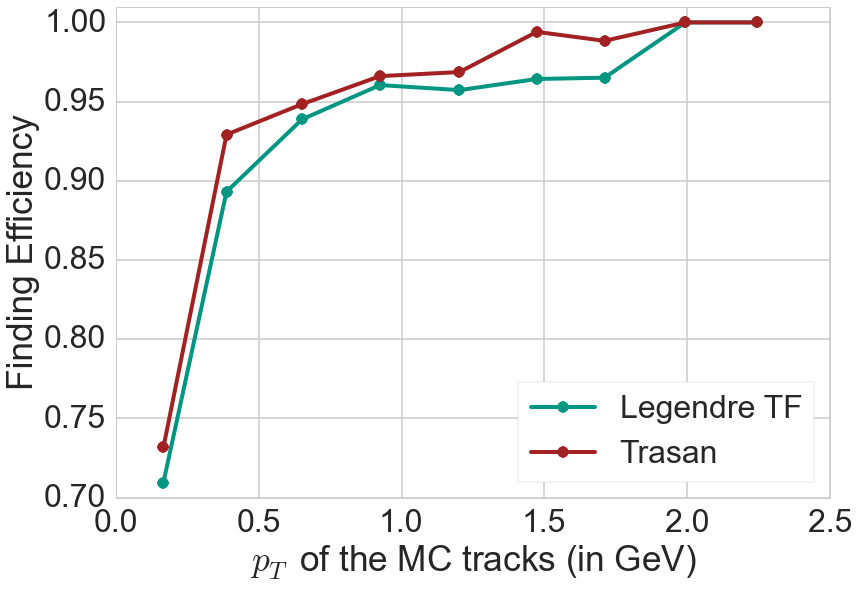
\includegraphics[width=0.48\linewidth]{figures/workflow/legendre_pt.png}
  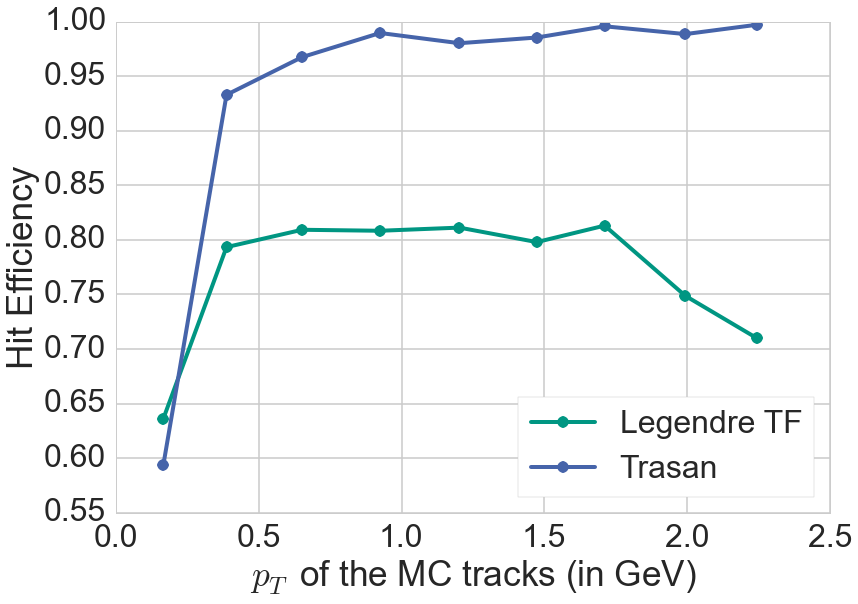
\includegraphics[width=0.48\linewidth]{figures/workflow/legendre_hit.png}
  \caption{Finding and hit efficiency over $p_T$ for the Legendre track finder and trasan. In both categories, the legendre track finder performs worse than the reference implementation.}
  \label{fig-legendre-finding-efficiency}
  % Using InputData 2
  % Final
\end{figure}

As described in chapter~\ref{chapter-theory}, the Legendre tracking algorithm is adversely affected by large distances of the tracks to the origin (typical for secondaries), which is shown in figure~\ref{fig-legendre-d0}.

\begin{figure}
  \centering
  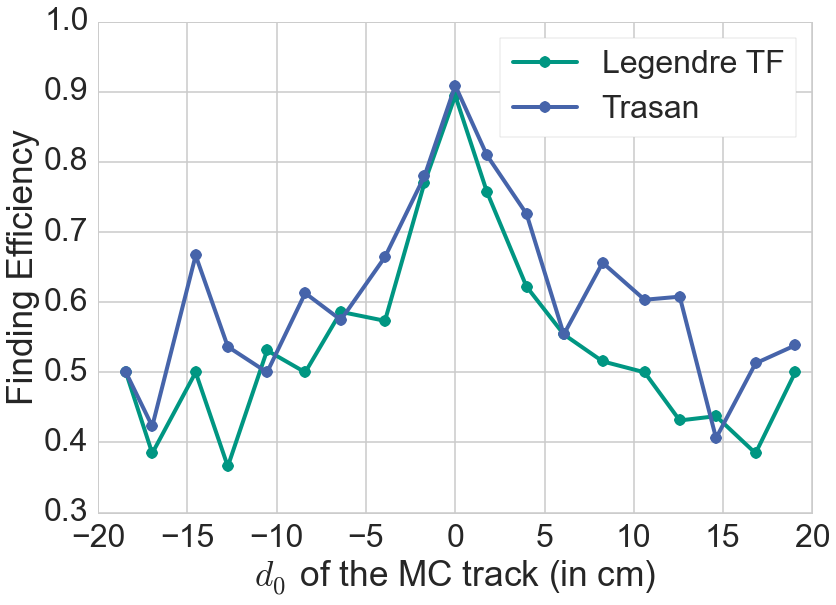
\includegraphics[width=0.7\linewidth]{figures/workflow/legendre_d0.png}
  \caption{Finding efficiency over $d_0$ for the Legendre track finder and trasan. The distance $d_0$ is the one of the helix parameters and describes the minimal distance from the track to the interaction point in the $r$--$\phi$-projection.}
  \label{fig-legendre-d0}
  % Using InputData 2
  % Final
\end{figure}

In addition to the hit efficiency, also the hit purity plays an important role for the later physics analyses as wrong hits in a track can reduce the resolution. As can be seen, the hit purity is on a rather high level (above 94 \%) and drops as expected for low momentum particles. In comparison to trasan however, the hit purity should be increased further.

\begin{figure}
  \centering
  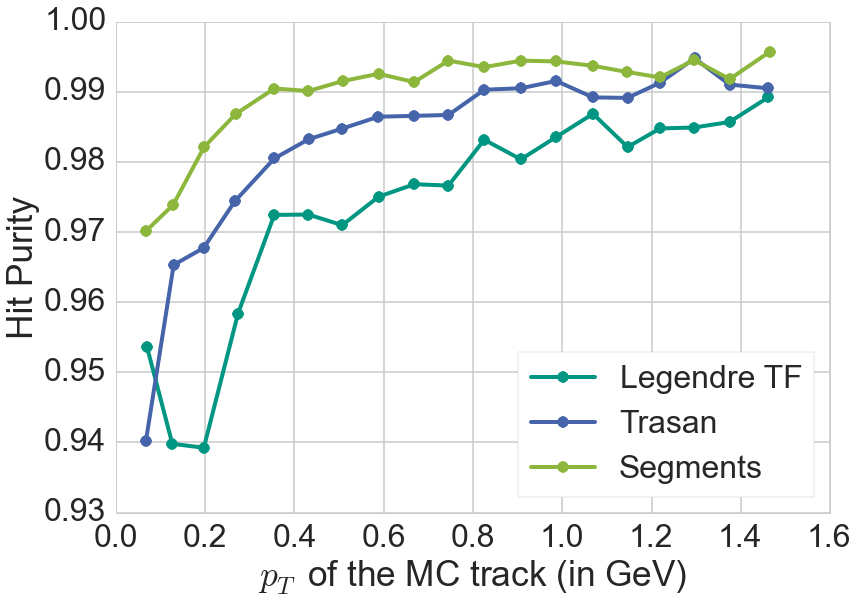
\includegraphics[width=0.7\linewidth]{figures/workflow/segment_purity.png}
  \caption{Hit purity over $p_T$ of the related MC track for the Legendre track finder, the segments from the local track finder and trasan. The hit purity is calculated as the number of correct hits in a track divided by the full number of hits.}
  \label{fig-legendre-purity}
  % Using InputData 2
  % Final
\end{figure}


\paragraph{Local Track Finder}

As seen in table~\ref{tab-old-implementation-results}, the local track finder does not lead to good results when using the produced tracks. Therefore, only the produced segments in the first step of the automaton finder are used in the following. The segments however, as seen in figure~\ref{fig-legendre-purity}, have a very high purity. Also, if not combining them to tracks, more or less every MC particle is found by one or more segments (see figure~\ref{fig-segments-efficiency}) not depending on $d_0$ as the Legendre track finder. This high efficiency and purity can be used for the stereo finder (section~\ref{section-stereo}) and for the combination of the two track finders (section~\ref{section-combiner}).

\begin{figure}
  \centering
  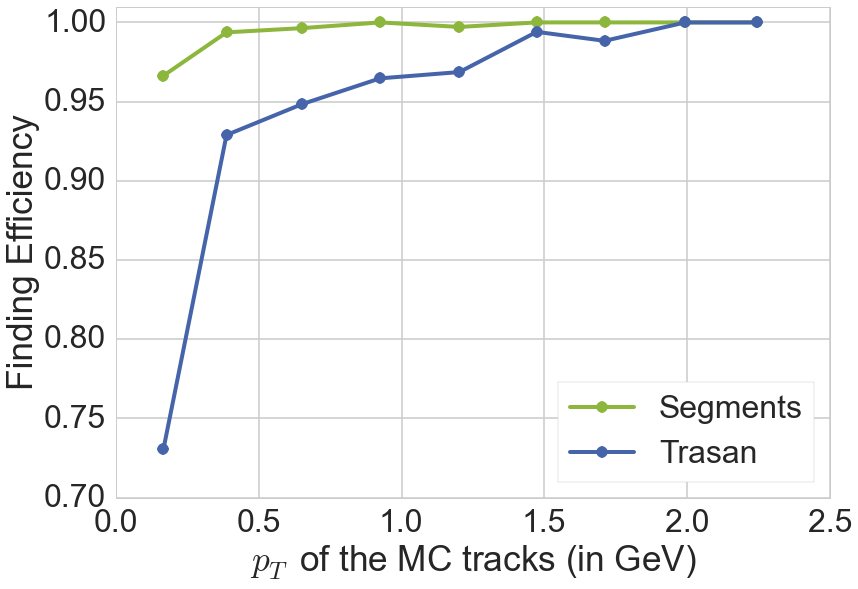
\includegraphics[width=0.48\linewidth]{figures/workflow/segments_pt.png}
  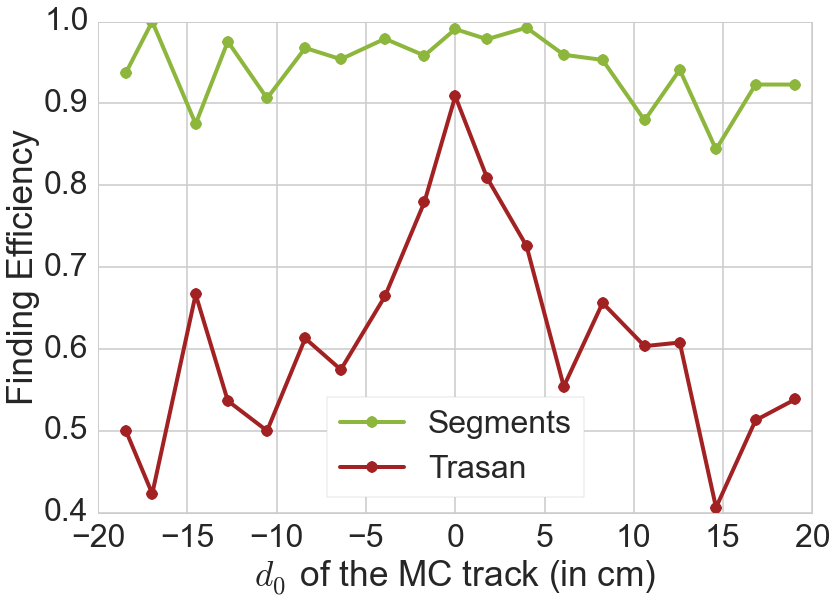
\includegraphics[width=0.48\linewidth]{figures/workflow/segments_d0.png}
  \caption{Finding over $p_T$ and $d_0$ for the segments from the automaton track finder and trasan. The local track finder has more or less no dependency on momentum or distance to the interaction point.}
  \label{fig-segments-efficiency}
  % Using InputData 2
  % Final
\end{figure}

\section{The \texttt{TrackFindingCDC} Package}
As presented in the section before, the two track finding algorithms have different characteristics. To use the benefits of both, a combined approach is suited best. The proposed workflow as a result of the analysis done in this thesis is presented simplified in figure~\ref{fig-workflow}. The idea is to run both track finders on the same (full) set of hits and combine the resulting tracks/segments afterwards. Another solution is to use only the hits that are not already used by the first track finder in the second one. The proposed approach has an increased computing time in contrast to this solution but has some other advantages: 
\begin{itemize}
 \item If a track is found by both track finders, the probability of it being a fake is very small.
 \item If a track is only found partly by the first track finder, the second algorithm will probably not find the rest as only some hits are unused. When both track finders use the full set of hits, the combined tracks include most of the hits of a track.
 \item Both track finder can be optimized independently. It is even possible to run only one of them to save computing time or for special detector setups (e.g. for cosmic runs) without changing much in the software configuration.
\end{itemize}

\begin{figure}
  \centering
  \begin{tikzpicture}[thick]
    \node[module] (simulation) {Simulation or Experiment};
    \node[module, below=1 of simulation] (background) {Background Hits Filter};
    \draw[vecArrow] (simulation) -- (background) node [midway, anchor=west] {CDC Hits};
    \node[module, below right=1.8 of background] (local) {Local Track Finder};  
    \node[module, below left=1.8 of background] (global) {Global Track Finder};  
    \draw[vecArrow] (background) -- (local) node [midway, auto=false, anchor=south, sloped] {CDC Hits};
    \draw[vecArrow] (background) -- (global) node [midway, auto=false, anchor=south, sloped] {CDC Hits};
    \node[module, below right=1.8 of global] (combiner) {Segment and Track Combiner};  
    \draw[vecArrow] (local) -- (combiner) node [midway, auto=false, anchor=south, sloped] {Segments};
    \draw[vecArrow] (global) -- (combiner) node [midway, auto=false, anchor=south, sloped] {Tracks};
    \node[module, below=1 of combiner] (fitter) {Track Fitter};
    \draw[vecArrow] (combiner) -- (fitter) node [midway, auto=false, anchor=west] {Tracks};
  \end{tikzpicture} 
 \caption[Proposed workflow in the CDC tracking]{The proposed workflow and combination of the two track finders in the CDC detector. The green boxes refer to one or a few modules. The arrows describe parts of the data flow between the modules. For clarity not all necessary parts are shown here.}
 \label{fig-workflow}
\end{figure}

For better interconnectivity between the track finders, they share a large code basis including common data objects and a common module system. Combining the code basis of the two track finders was also part of this thesis. The common software design consists e.g.\ of a common singleton (called \texttt{CDCWireHitTopology}) saved in the data store which is responsible for storing the used-flag of the CDC hits and their connection to other objects (like clusters or segments). Also the in- and output of all tracking modules in the CDC is handled by shared code which makes changes in the data flow much easier.

Figure~\ref{fig-workflow2} shows the same workflow as presented in figure~\ref{fig-workflow} (except the simulation and the track fit), but now with the correct module names and the relevant data flow. The \texttt{CDCWireHitTopology} singleton is not part of the modules but gets used by all modules to check the usage flag and the geometrical information of the wire hits. The modules in the path are described in the following in more detail.

\begin{description}
  \item[Wire\-Hit\-Topology\-Preparer] This module receives the simulated or measured hit information from the CDC detector and connects it with the geometrical information from a database. All hits together with configurable flags are saved in the wire hit topology object which is stored as a persistent object in the data store.
  \item[Segment\-Finder\-CDC\-Facet\-Automaton\-Dev] The module is the first part of the local track finder as described in chapter~\ref{chapter-theory}. As the clusterizer is one part in the cellular automaton used in this algorithm, it is -- apart from creating segments -- also used for separating signal and background hits. This filter is described in section~\ref{section-background}. As all CDC tracking modules communicate over the wire hit topology object, the background flag is propagated to all other modules. The rest of the module was not developed during this thesis and is described elsewhere~\cite{oliver}.
  \item[CDC\-Legendre\-Tracking] Running the axial Legendre track finder with the quad tree search is done in this part as described also in chapter~\ref{chapter-theory}. It uses the full wire hit set (except the background hits). It has also some post-processing steps included directly after the search, which were analyzed and improved in this thesis.
  \item[Track\-Quality\-Asserter\-CDC] Although all track finding algorithms are highly optimized, there is a need for quality improvement tools for the resulting track candidates. To make this step configurable for later adjustment and to share the code basis between the algorithms, tools for track corrections were developed in this thesis (see section~\ref{section-quality}). They can be used in the other modules directly or via this module which is used in two positions in the path with different configurations.
  \item[Stereo\-Hit\-Finder\-CDC\-Legendre\-Histogramming] After the axial track finder created tracks, they get used in this module to add stereo hits with a quad tree search. This module was rewritten from scratch in this thesis and is described in section~\ref{section-stereo}.
  \item[Segment\-Track\-Combiner\-Dev] The final step (except for quality improvements) is the combination of the results of the global and local track finder which is handled by this module. It was created during this thesis and is presented in section~\ref{section-combiner}.
\end{description}

\begin{figure}
  \centering
  \begin{tikzpicture}[thick]
    \node[module, text width=12em] (hits) {{Wire\-Hit\-Topology\-Preparer}};
    \node[module, below=1 of hits, text width=12em] (segment) {{Segment\-Finder\-CDC\-Facet\-Automaton\-Dev}};
    \node[module, below=1 of segment, text width=12em] (axial) {{CDC\-Legendre\-Tracking}};
    \node[module, below=1 of axial, text width=12em] (quality1) {{Track\-Quality\-Asserter\-CDC}};
    \node[module, below=1 of quality1, text width=12em] (stereo) {{Stereo\-Hit\-Finder\-CDC\-Legendre\-Histogramming}};
    \node[module, below=1 of stereo, text width=12em] (combiner) {{Segment\-Track\-Combiner\-Dev}};
    \node[module, below=1 of combiner, text width=12em] (quality2) {{Track\-Quality\-Asserter\-CDC}};
    
    \node[cloud, right=3 of hits] (topo) {{CDCWireHitTopology}};
    
    \draw[vecArrow] (hits) -- (topo) node [midway, anchor=south, sloped, auto=false] {All CDC Hits};
    \draw[vecArrow] (topo) -- (segment) node [midway, anchor=south, sloped, auto=false] {All CDC Hits};
    \draw[vecArrow] (segment.east) -- (topo.south) node [midway, anchor=north, sloped, auto=false] {Filtered CDC Hits};
    \draw[vecArrow] (topo.south) -- (axial.east) node [midway, anchor=north, sloped, auto=false] {Filtered CDC Hits};
    \draw[vecArrow] (axial) -- (quality1) node [midway, anchor=west] {Axial Tracks};
    \draw[vecArrow] (quality1) -- (stereo) node [midway, anchor=west] {Corrected Axial Tracks};
    \draw[vecArrow] (stereo) -- (combiner) node [midway, anchor=west] {Full Tracks};
    \draw[vecArrow] (combiner) -- (quality2) node [midway, anchor=west] {Combined Tracks};
    \draw[vecArrow] (segment.west) to[out=-150, in=150] node [midway, anchor=east] {Segments} (combiner.west) ;
  \end{tikzpicture} 
 \caption[Detailed workflow in the CDC tracking]{The detailed workflow for the track finding procedure for the CDC detector with the correct names of the modules as in the software. The green boxes refer to one module. The red ellipse is an object on the data store. Some dependencies between the modules are shown as arrows.}
 \label{fig-workflow2}
\end{figure}

\section{The Background Hit Finder} \label{section-background}
The beforementioned track finders are tuned to not pick up background hits into a found track candidate or even form a candidate with background hits only. Nevertheless, the algorithms are not perfect and even a single background hit per track can lead to a reduced momentum resolution or can even cause the fit to fail completely. Together with the reduced combinatorics and therefore reduced computing time when throwing away unusable hits, there is the need to distinguish between signal and background hits even before the tracking starts. This is the purpose of the background hit finder described in this section. The background hit finder is part of the \texttt{SegmentFinderCDCFacetAutomatonDev} module but is described here as a standalone part.

For deciding if a hit is to be used in the track finder, the module uses implemented filters. As these filters are used widely in the whole CDC tracking framework, they are described here in more detail. To filter out bad hits, not only the information of one hit but the information of the clusters constructed in the local track finder is used. As described in chapter~\ref{chapter-theory}, they are created by clusterizing all CDC hits in such a way that one cluster includes the maximum number of connected hits. Two hits are called connected if there is no non-fired wire geometrically between them. Because of the modular framework and the reusable \texttt{CDCWireHitTopology}, it is possible to run the local track finder with the clusterizer before the Legendre track finder and propagate the background information to the following tracking algorithms. 

Figure~\ref{fig-clusters} in chapter~\ref{chapter-theory} shows an event display in the $r$--$\phi$-plane with the clusters drawn in different colors. Figure~\ref{fig-cluster-hit-purity} shows the hit purity of clusters from typical events. The hit purity is computed as the ratio between the number of hits in a cluster which belong to a signal track divided by the number of all hits (including the ones coming from background only). As can be seen clearly in this histogram, a cluster is either full of background or full of signal hits - for that throwing away a background cluster does not involve deleting hits that are needed for signal tracks. However, using clusters instead of single hits in the filter has the advantage of more information about the neighborhood of the hits.

\begin{figure}
  \centering
  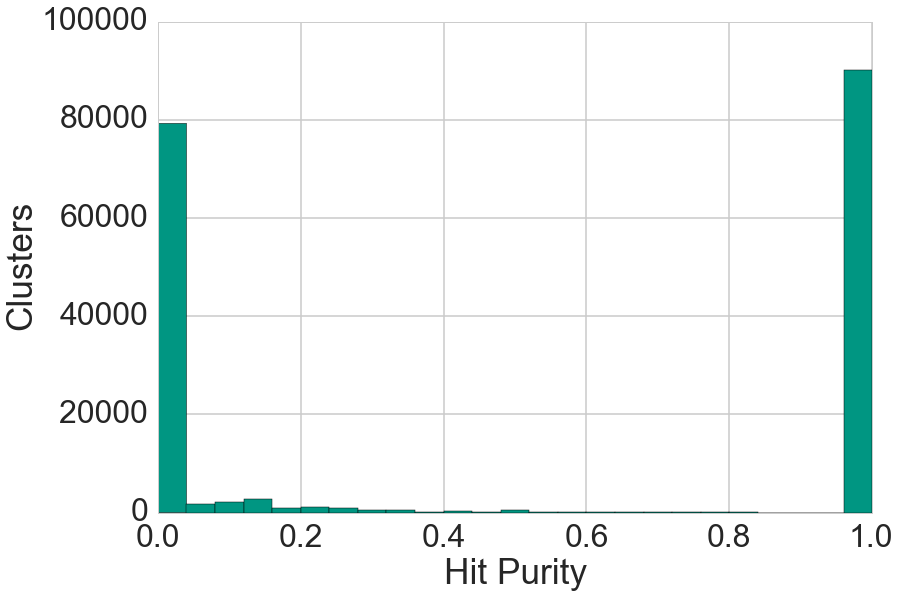
\includegraphics[width=0.7\linewidth]{figures/workflow/cluster_purity.png}
  \caption{Histogram of the hit purities (ratio between signal hits to all hits in a cluster) of the found clusters by the clusterizer as part of the local track finder algorithm. As the clusters are either purely signal or purely background, they can be kept or thrown away as whole objects.}
  \label{fig-cluster-hit-purity}
  % Does not matter
  % Final
\end{figure}

In every event, each formed cluster is passed to the filter with the chosen parameters to decide whether to use the hits in this clusters for track finding or not. This filter can return every number as a result or a flag for indicating that the cluster should not be used further for track finding as it is marked as background by the filter. The number can be used to describe additional information, e.g.\ the probability of the cluster to be signal.

The filter design is very general and leaves the possibility open to compare many different filters. For the background filter as well as for many other used filter in the CDC tracking, five filters are implemented which can be selected by using module parameters. These filters are:

\begin{description}
  \item[BaseFilter] is a filter that neglects every item. It is the base object for every other filter and is rarely used in production.
  \item[AllFilter] is the counterpart of the \texttt{BaseFilter} and accepts all items. It can be used for testing purposes to make a filter fully transparent.
  \item[SimpleFilter] is a filter based on self-implemented cuts. The variables to cut depend on the planned usage of the filter and need to be implemented by the user.
  \item[TMVAFilter] is based on a trained boosted decision tree\footnote{TMVA~\cite{tmva} is an acronym for Toolkit for Multivariate Data Analysis in the ROOT framework.}. It passes the variables defined in a so-called \texttt{VarSet} to the BDT and returns a result between 0 and 1. If the result is lower than a certain cut definable on runtime, the \texttt{TMVAFilter} discards the item -- otherwise the result of the BDT is returned. The variables can be freely defined by the user. In most of the cases, the separating force of a well-trained BDT exceeds the one of a simple cut-based filter.
  \item[RecordingFilter] returns only a single constant defined on runtime independent on the input and can therefore not directly be called a filter. Instead, its purpose is to write the same variables as the \texttt{TMVAFilter} uses together with a truth information of every incoming item into a ROOT \texttt{TNTuple}. The output file with this \texttt{TNTuple} can later be used to train the BDT of the \texttt{TMVAFilter} to categorize according to the truth information. This filter can of course only be used on simulated data.
  \item[MCFilter] filters the items according to the truth information compiled with the MC information that is also used in the recording filter.
\end{description}

As an example for the mentioned \texttt{VarSet}, the variables for distinguishing the background clusters from the signal clusters is described in table~\ref{tab-varset-cluster}. The truth information used for the BDT training is also described there. It is not always obvious why the described variables can help to separate between background and signal clusters. This is why typical signal and background clusters are shown in figure~\ref{fig-cluster-versus}. As can be seen in the figure, background clusters have a different shape as signal clusters. Particles creating signal hits pass almost straightly through the detector leaving behind a defined, long-shaped trace of hits whereas background hits get created in a single spot forming more circular-shaped clusters (if they have more than one hit at all). This shape information can be seen in the number of neighbors as well as in the averaged distance to the superlayer center. The latter is zero for most of the signal clusters as the particles go through the whole superlayer whereas background hits do not span the whole section. As the background clusters are made of hits coming from stochastically distributed processes, the parameters of the hits like time information (which gets transformed to the drift length) or deposited energy (which is encoded in the ADC count) are probably randomly distributed. This is why the first two momenta of the distributions (mean and variance) of these variables in a cluster are also taken into account.

\begin{figure}
  \centering
  \begin{minipage}{0.58\linewidth}
    \centering
    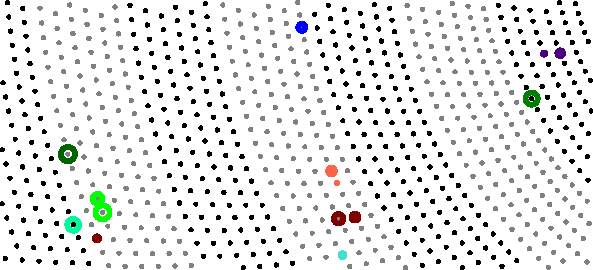
\includegraphics[scale=0.8]{figures/workflow/cluster_display_background.pdf}
  \end{minipage}
  \begin{minipage}{0.4\linewidth}
    \centering
    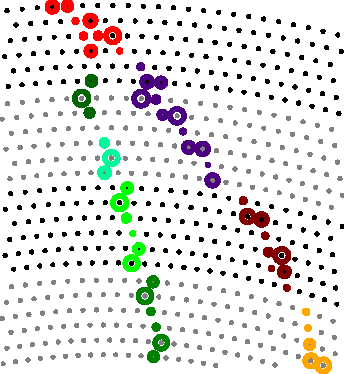
\includegraphics[scale=0.8]{figures/workflow/cluster_display_signal.pdf}
  \end{minipage}
  \caption{Detailed view of a full event display (cf. figure \ref{fig-clusters} in chapter~\ref{chapter-theory}) with found clusters colored differently for better visualization. The left subfigure shows background clusters, whereas the right one shows clusters with hits from simulated signal particles. The differences in the described variables like shape, number or distance can be seen.}
  \label{fig-cluster-versus}
  % Does not matter
  % Final
\end{figure}


\begin{table}
  \centering
  \begin{tabular}{p{0.35\linewidth}p{0.60\linewidth}} \toprule
   Variable Name & Description \\ \midrule
   \verb+is_stereo+ & Boolean variable if the cluster is in a stereo superlayer or not. Has no separating force by itself but only in combination with other variables. \\ \midrule 
   \verb+superlayer_id+ & The index of the superlayer counted from the most inner superlayer outwards. As the \verb+is_stereo+ variable, it should be used in combination with other variables.\\ \midrule 
   
   \verb+size+ & The number of hits combined to a cluster. This variable by itself has the best separation power among all variables, as background hits occur most likely as disconnected hits whereas signal hits are connected to others in the track they form.  \\ \midrule 
   
   \verb+total_number_of_neighbors+ & \multirow{2}{*}[-1.5pt]{\begin{minipage}{\linewidth} The number of neighbors for one hit is the count of hits in the direct surrounding of a wire hit and can therefore be at most six (as can be seen in figure~\ref{fig-sense-wires} in chapter~\ref{chapter-ex}). The sum of all neighborhood numbers for all hits in the cluster and the total number divided by the number of wire hits are used. \end{minipage}} \\[5ex] \cmidrule{1-1}
   \verb+mean_number_of_neighbors+ & \\[5ex] \midrule 
   
   \verb+total_drift_length+ & \multirow{3}{*}[-1.5pt]{\begin{minipage}{\linewidth} The drift length is a function of the measured time delta between the initial $\Pem\Pep$-collision and the moment the drifting electrons touch the sense wires. The sum over all hits in a cluster, the averaged drift length and the variance is used. \end{minipage}} \\[1ex] \cmidrule{1-1}
   \verb+mean_drift_length+ & \\[1ex] \cmidrule{1-1}
   \verb+variance_drift_length+ & \\[1ex] \midrule 
   
   \verb+total_inner_distance+ & \multirow{3}{*}[-1.5pt]{\begin{minipage}{\linewidth} The inner distance is the geometrical difference between the wire position in the $r$--$\phi$-plane and the interaction point. For stereo hits, the position for $z = 0$ is chosen. \end{minipage}} \\[1ex] \cmidrule{1-1}
   \verb+mean_inner_distance+ & \\[1ex] \midrule
   \verb+distance_to_+ \verb+superlayer_center+ & Additionally to calculating the distance to the interaction point, the averaged radial distance from the wire hits to the center of the superlayer the cluster lays in is calculated. \\ \midrule 
   
   \verb+total_adc_count+ & \multirow{3}{*}[-1pt]{\begin{minipage}{\linewidth} Together with the time delta of the incoming drifting electrons each sense wire measures also the number of electrons that were ionized in the drift cells. The ADC count is the digitized value of this number. \end{minipage}} \\ \cmidrule{1-1}
   \verb+mean_adc_count+ & \\ \cmidrule{1-1}
   \verb+variance_adc_count+ & \\ \midrule
   \verb+truth+ & A cluster is counted as signal if more than 80 \% of the contained hits belong to a simulated MC particle (and not to background). As the number of hits in one cluster is mostly very small, this implies that all hits must be from a signal track for most of the cases. \\ \bottomrule
  \end{tabular}

  \caption{The variables used for the classifier to separate background from signal clusters (and hits). Additional information on some of the variables can be found in the text.}
  \label{tab-varset-cluster}
\end{table}

After the recording and the training procedure (which is handled by Python scripts) the \texttt{TMVAFilter} with the mentioned \texttt{VarSet} can be used. Figure~\ref{fig-result-background-hit-finder} shows the receiver operating characteristic curve (ROC) and the distribution of the BDT result for the training and the testing set of clusters. As can be seen, the BDT has a very good separation power between background and signal clusters. As the output distributions for testing and training data set are very similar, there is no overtraining visible.

\begin{figure}
  \centering
  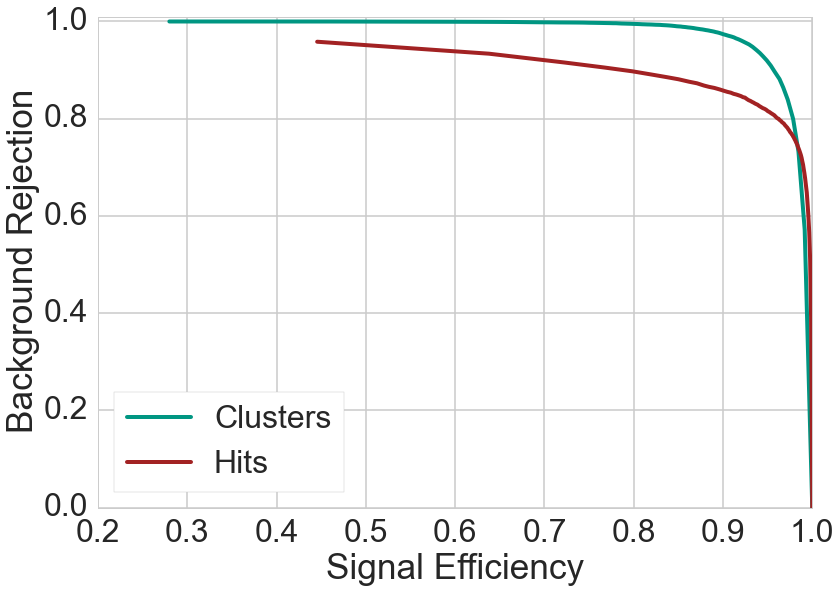
\includegraphics[width=0.48\linewidth]{figures/workflow/background_hit_finder_roc.png}
  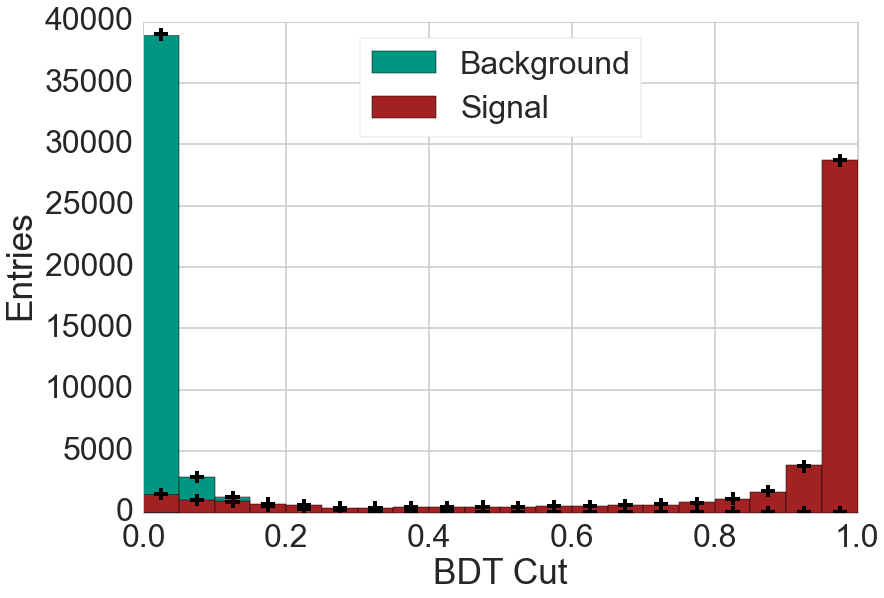
\includegraphics[width=0.48\linewidth]{figures/workflow/background_hit_finder_overtraining.png}
  \caption{The left plot shows the background rejection over the signal efficiency (so-called ROC curve) for the trained BDT which distinguishes between signal and background clusters. Also shown is the ROC curve recalculated using the hits in each cluster. As the number of hits in each cluster is not constant, the two curves differ. The right histogram describes the distribution of the output variable of the BDT for signal and background clusters in the testing (cross markers) and the training (bars) data set. No overtraining is visible as the distributions match perfectly well.}
  \label{fig-result-background-hit-finder}
  % Does not matter
  % Final
\end{figure}

By applying a cut on the BDT output the background hits can be marked and do net get used in the following tracking routines. How this cut is chosen depends on the desired optimization. A lower cut can include many background hits but does not throw away signal hits keeping the fake rate as well as the hit efficiency high. A harsher cut however can increase the finding efficiency as the combinatorics are reduced and the probability to collect background hits is lower. Figure~\ref{fig-result-background-hit-finder2} shows the figures of merit of the axial Legendre track finder with different cuts on the BDT output. Especially the fake rate can be reduced by using the background hit finder. Figure~\ref{fig-hits-numbers} shows the number of signal/background hits and clusters for different cut values. As the number of background clusters/hits is reduced with higher cut values, the combinatorics are reduced as well. This can be seen in figure~\ref{fig-performance-clusters}, where the computation time of the both track finder algorithms is shown. In the following, a cut value of 0.2 is used.

\begin{figure}
  \centering
  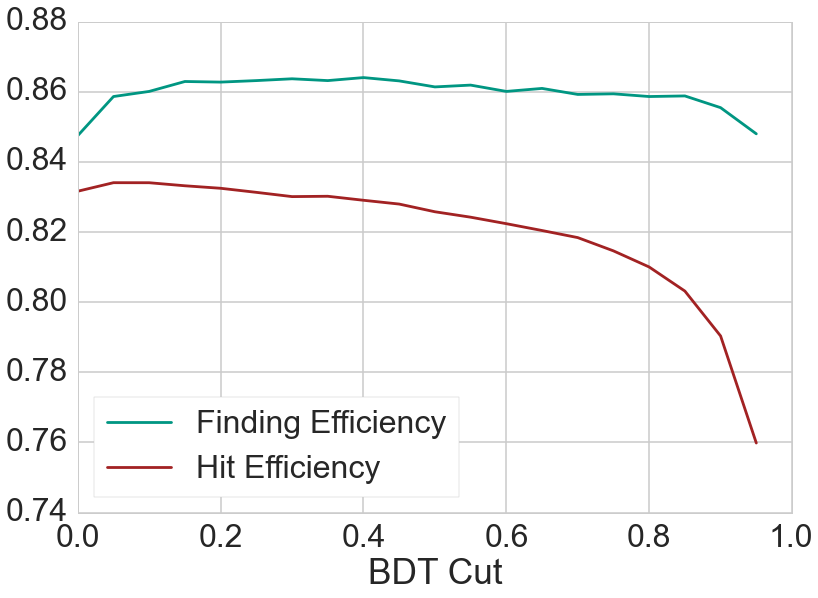
\includegraphics[width=0.48\linewidth]{figures/workflow/background_hit_finder_efficiency.png}
  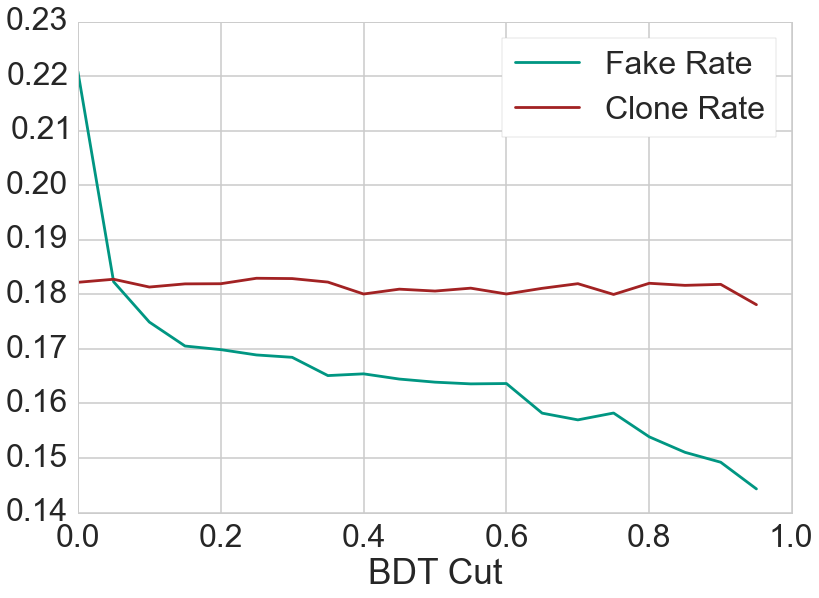
\includegraphics[width=0.48\linewidth]{figures/workflow/background_hit_finder_rate.png}
  \caption{Figures of merit of the Legendre track finder (without combination with the automaton track finder and without final track quality corrections) for different cut values on the BDT in the background hit finder. The rate of fakes could be reduced drastically. The finding efficiency and the clone rate stay almost the same. When the cut on the BDT output is to tight, the hit efficiency is decreased.}
  \label{fig-result-background-hit-finder2}
  % Calculated with InputData 2
  % Final
\end{figure}

\begin{figure}
  \centering
  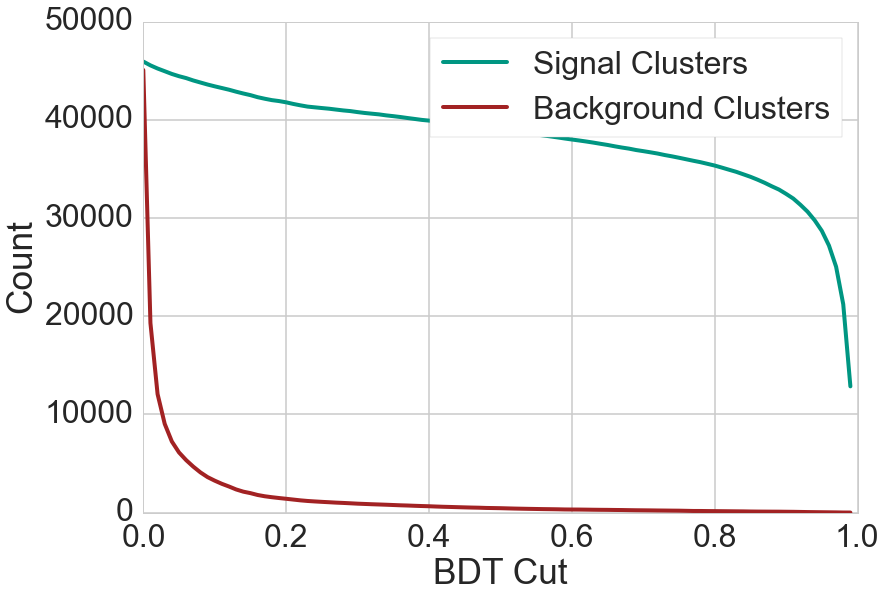
\includegraphics[width=0.48\linewidth]{figures/workflow/number_of_clusters.png}
  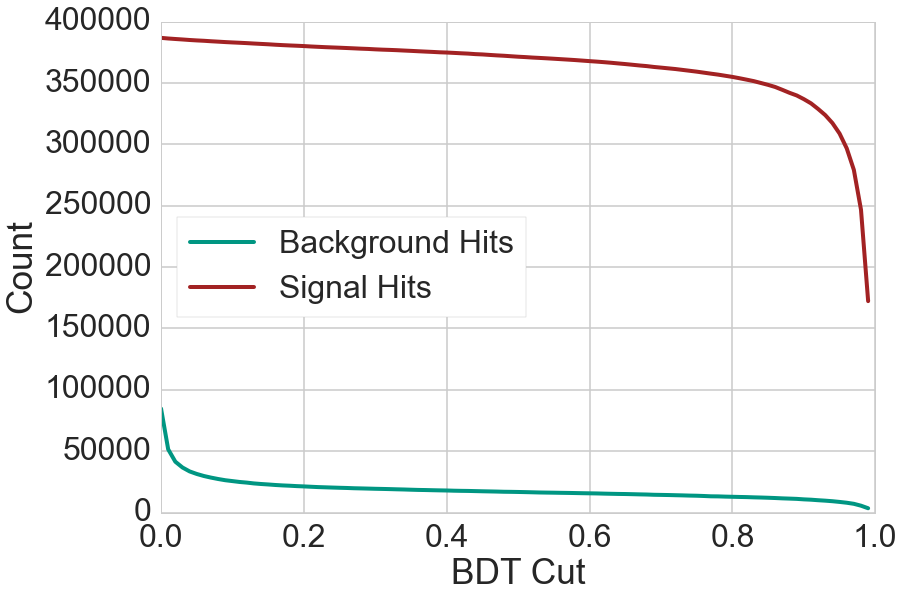
\includegraphics[width=0.48\linewidth]{figures/workflow/number_of_hits.png}
  \caption{Number of signal/background clusters/hits after a cut on the BDT output. The number of signal hits stays more or less the same for the lower cut value region whereas the number of background hits decreases.}
  \label{fig-hits-numbers}
  % Does not matter
  % Final
\end{figure}

\begin{figure}
  \centering
  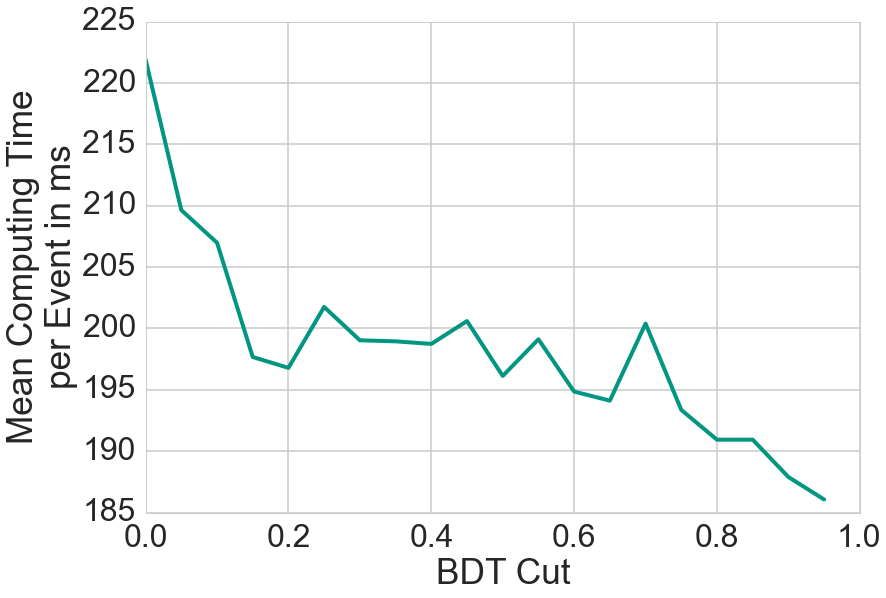
\includegraphics[width=0.7\linewidth]{figures/workflow/background_hit_finder_performance.png}
  \caption{Averaged computing time per event of the two track finder algorithms (local and global) in sum (including the changes as described in the following sections) for different cut values on the BDT output. Except for statistical fluctuations, the computing time decreases with tighter cuts, as the total number of hits gets smaller.}
  \label{fig-performance-clusters}
  % Does not matter
  % Final
\end{figure}

% \section{Improvements on the Axial Legendre Track Finder}
% Is already very good and advanced. 

% \subsection{The class \texttt{QuadTreeProcessorTemplate}}
% \subsection{Postprocessing after the track finding}
% \subsection{Results}
% Timing

\section{Improvements on the Stereo Legendre Hit Finder} \label{section-stereo}

The previous implementation of the stereo hit finder yielded good finding and hit efficiencies with an acceptable fake and clone rate. However, the module was partly built with legacy code and had a very bad computing performance as the processing time of the stereo finder was about 20 times higher than the axial finder. Instead of refactoring the module, it was rebuilt from scratch during this thesis using the common code basis for all track finder algorithms in the CDC and the same quad tree structure as the axial hit finder. Additionally, a refined stereo position calculation was implemented using the already provided methods from the framework and a second coordinate axis was introduced in the quad tree. Before, the stereo hit finder used only the $\lambda$ angle for a histogramming method whereas in the new module the the slope in the $s$--$z$-plane (which is the tangent of $\lambda$) and $z_0$ are used as described in chapter~\ref{chapter-theory}. Because of an introduced caching method, the computation could be speed up by a factor of approximately 200. The algorithm is described in the next paragraph whereas the results in comparison to the old implementation are shown after that.

\subsection{Implemented algorithm}

The stereo hit finding algorithm consists of three stages, which are repeated for every found axial track. In between the iterations for every track, the found hits are marked to not use them twice. The steps are in detail:
\begin{zlist}
  \item \textit{Fill a list of hits and pass them to the quad tree.} All non-used stereo hits from the \texttt{CDCWireHitToplogy} (except background hits) are used to create a list of reconstructed hits. These hits have a cached travel distance $s$ and a $z$ position, that is calculated using the axial track. It is chosen in such a way, that the trajectory in the $r$--$\phi$-plane touches the drift circle of the wire hit perfectly. As there are inherently two possible orientations of the hit -- left or right -- there are two items in the list for each wire hit. A check if the travel distance is negative (which happens for hits laying on the other side of the CDC than the track) and if the reconstructed $z$ value is outside of the CDC boundaries is applied. 
  \item \textit{Quad tree search for the best candidate.} The $\tan \lambda$ and the $z_0$ values of the passed items in the list are used in a quad tree search. For this, a line in the $s$--$z$-space is constructed with the slope $\tan \lambda$ going through $(0, z_0)$. An item belongs to a quad tree bin if and only if this line goes through the bin borders exactly twice (which can easily be checked using the mean value theorem). As only one single axial track is used for reference at a time, only the highest bin in the quad tree search is used as a result. If both the right and left hypothesis of a hit are in the resulting bin, the one orientation closer to the trajectory is used.
  \item \textit{Add the found hits to the axial track and clear the quad tree.} After the search is finished, the found stereo hits are added to the axial hits and the track hits are sorted correctly. A line fit is performed to extract the $z$-information of the trajectory. In the end, the quad tree is cleared and prepared for the next track.
\end{zlist}

Both quad tree algorithm implementations currently available in the framework can be used in the module. As they both use the same principles, only the results of one implementation are shown. Additionally, as items for the list passed to the quad tree not only stereo wire hits but also stereo segments coming from the local track finder can be used. Instead of checking if the line in the $s$--$z$-plane intersects with the quad tree bin for a single hit, all hits in the segment are checked for. If the lines of more than 70 \% of the hits in a segment intersect with a quad tree bin, the whole segment is counted in in this bin with the number of intersecting hits as a weight. As the segment already gives right--left-information to the wire hits, only the whole orientation can be flipped (and is flipped when the charge of the track and the segment differ). Using segments instead of hits has some benefits: as the hit purity of the segments is rather high, adding whole segments instead of single hits can improve the hit efficiency and purity of the stereo tracks. Also, as the number of segments is much smaller than the number of hits, the combinatorics in the quad tree search are reduced resulting in a smaller quad tree level and a smaller computing time. The drawback, however, is that single wrong or wrongly reconstructed\footnote{As the $z$-position reconstruction depends heavily on the trajectory parameters in the $r$--$\phi$-plane, the calculation can give wrong results when these parameters are off because of energy loss or low hit purity of the axial track.} hits can influence the segment quite much and if a whole segment is lost because of a few wrong hits, the hit efficiency can be reduced severely.

\subsection{Results}

The two operation modes in the new stereo hit finder module (with bare wire hits or with segments) can be compared to the old stereo hit finder implementation and also with the reference implementation trasan from Belle. The figures of merit and the computation time per event are shown in table~\ref{tab-stereo-results} together with the finding and hit efficiency as a function of $p_T$ in figure~\ref{fig-stereo-results}. 

\begin{table}
  \caption{Table showing the figures of merit for the two new implementations (using hits or segments), the old implementation and trasan. As trasan is responsible for adding axial and stereo hits, the computing time for stereo only can not be deduced.}
  \centering
  \begin{tabular}{lcccc} \toprule
    & Hits & Segments & Old Implementation & Trasan \\ \midrule
    Finding Efficiency & 86.28 & 85.19 & 83.17 & 85.53 \\
    \quad on Primaries & 92.32 & 91.26 & 89.94 & 91.49 \\ 
    Hit Efficiency     & 83.23 & 78.23 & 74.03 & 81.93 \\
    \quad on Primaries & 88.96 & 83.26 & 78.22 & 87.25 \\ 
    Clone Rate         & 14.33 & 15.30 & 7.69  & 19.50 \\
    \quad on Primaries & 7.63  & 8.14  & 4.71  & 17.17 \\ 
    Fake Rate          & 18.60 & 18.44 & 26.82 & 15.95 \\ 
    Wrong hits per Track & 2.10 & 2.46 & 2.69  & 1.09  \\
    Time per Event in ms & 36.54 & 34.65 & 635.05 & 419.50 \\ 
    \quad only Stereo Finder & 2.79 & 1.27 & 578.76 & - \\ \bottomrule
  \end{tabular}
  \label{tab-stereo-results}
  % On Input Data 2
  % Trasan should be the same as in first table. Old should be the same as in first table (Legendre).
  % Hits should be the same as in combination table below.
  % Trasan final, Old Implementation final
  % with track quality asserter after Axial!
  % Final
\end{table}

\begin{figure}
  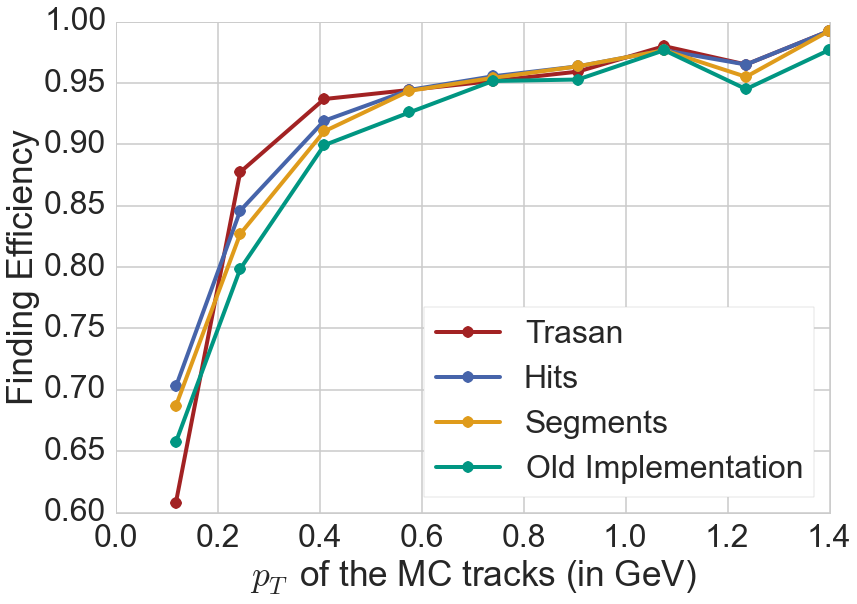
\includegraphics[width=0.48\linewidth]{figures/workflow/stereo_finding_efficiency.png}
  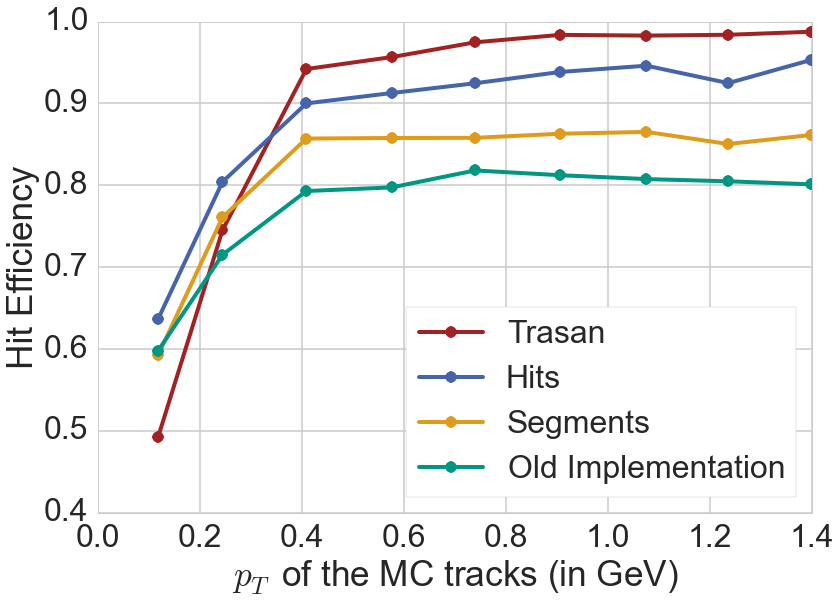
\includegraphics[width=0.48\linewidth]{figures/workflow/stereo_hit_efficiency.png}
  \caption{Finding (left) and hit (right) efficiency of the four tracking algorithms with axial and stereo finding. Although the two new implementation look worse than the reference implementation trasan, it must be noticed that in the lower $p_T$ region there are much more particles present leading to a higher weight on these tracks.}
  \label{fig-stereo-results}
  % On Input Data 2
  % Final
\end{figure}

As can be seen, the figures of merit are enhanced by the newly written module and are now comparable or better than the reference implementation trasan. This is mainly because of the additional coordinate in the quad tree which handles track not coming from the interaction point. The computing time is much smaller which is mainly because of caching and optimized calculation procedures, e.g.\ by changing the coordinates in the Legendre space from $\lambda$ which needed heavy trigonometrical calculations to the much easier to calculate $s$--$z$-slope. Please keep in mind, that also some implementation details of the axial Legendre track finder have changed between the old and the new implementation.

The both implementations - using bare hits or segments in the quad tree - share most of their properties like a small execution time and a high finding efficiency with rather low clone rate. As described in the previous paragraph, the approach with using segments leads to a lower fake rate (because the probability of adding single wrong hits is rather low), but also to a lower hit efficiency as when using bare wire hits in the quad tree. The execution time per event is higher when using hits as expected, because the maximum level of the quad tree could be reduced when using segments because of the reduced combinatorics. 

The hit efficiency of the approach using segments can possibly be increased by using a more advanced method to make the decision if a segment belongs to a quad tree bin or not. Possibilities include 
\begin{zlist}
 \item non-quadratic or overlapping bins to include also segments where one or two wrongly reconstructed hits shift the overall segment position in the Legendre space,
 \item a smoothened cut by including also segments in a quad tree bin with less then 70 \% of the hits belonging into this bin, but with a much lower weight,
 \item different methods to make the decision, e.g.\ to use the information provided by the facets in each segment or to make a fit on the $s$--$z$ coordinates of all hits in a segment and use the results.
\end{zlist}

In the following, the stereo hit finder using reconstructed hits in the quad tree is used because of its higher hit and finding efficiency.

\section{The \texttt{SegmentTrackCombinerDevModule}} \label{section-combiner}

To increase the hit efficiency, the segments found by the local track finder and the tracks from the global track finder can be combined. This unifies the benefits of both track finder as the local track finder itself can not handle the combination of whole tracks well whereas the global track finder easily looses some hits of a track -- especially for secondary particles. Merging the two track finders has also another benefit: if all possible segments and tracks combinations are made, the remaining segments can be used to form new tracks and can help to fill the phasespace gaps of the Legendre track finder. Lastly, tracks without any matching segments are most likely fake tracks and can be deleted.

\subsection{Principle of the Segment Track Combiner}

The matching procedure between tracks and segments is a multi-step process including up to seven filters. In the default configuration, most of them are turned off because of their huge influence on the finding efficiency. The used filters are still under development and further analyses are needed. In the following, tracks refers to the result of the global track finder whereas segments describes the output of the local track finder. The algorithm consists of the following steps:
\begin{zlist}
 \item Creation of a fast segment and track lookup.
 \item First matching of segment and tracks that share one or more hits. \label{list-start}
 \item Deletion of fake segments. \label{list-fakes}
 \item Flagging of segments belonging to particles that probably can not be found by the global track finder (and can therefore not be matched).
 \item Matching of the remaining segments with the tracks or among themselves and then with the tracks (not used in the following). \label{list-second}
 \item Filtering of fake tracks in the made combinations.  \label{list-end}
 \item Cleanup of the lookup cache.
\end{zlist}

The steps (\ref{list-start}) - (\ref{list-end}) include one or more filters which consist mostly of a trained BDT as the one described for the background hit finder. Some of the steps are described in the following in more detail.

\paragraph{First Matching (step \ref{list-start})}
This filter is probably the simplest but best one in the combiner module. It combines every track with every segment sharing at least one hit (but not all hits of the segment, as these are trivial matches) and evaluates the pair with a trained BDT. This BDT uses variables describing the quality of the match, e.g.\ the distance between the hits or the trajectories of the segment and the track or a common fit. If the output value of the BDT is above a certain user-defined cut, the combination is kept. If there is only a single possible combination for a segment in a given superlayer, the hits of the segment are added to the matching track. If there are more than one possibility, only the one with the highest BDT output is used. The shared hits of the segment with all other tracks are removed from the tracks. Figure~\ref{fig-first-filter-count} shows the number of correct and wrong combinations passing the BDT for different cuts on its output. It can be seen, that the number of correct matches is higher than the number of wrong matches without the BDT cut already. The reason is the condition to share at most one hit which filters out many of the wrong combinations (but also some correct ones). Figure~\ref{fig-first-filter-fom} shows the influence of the filter to the the figures of merit, when applying only this  filter in the end of the full path of modules described in section~\ref{section-fom} (but without the track quality modules). As expected, the hit efficiency is highly dependent on the cut value. As a cut value of one corresponds to no added segment, the figures of merit for this cut correspond to the ones without the \texttt{SegmentTrackCombinerDevModule}. The hit efficiency can be increased by adding correct segments (cut values in the region 0.2 -- 0.8), but drops if too many wrong segments are added (0 -- 0.2). The fake rate and therefore the finding efficiency behave similarly. Finally, figure~\ref{fig-first-filter-fom} shows also the averaged number of wrong hits per track as a function of the BDT cut. It shows the same behavior as seen before as the number of wrong hits decreases with tighter cut values. In the following, a cut value of 0.75 is used which is a good trade-off between low clone and fake rate and high hit efficiency.

\begin{figure}
  \centering
  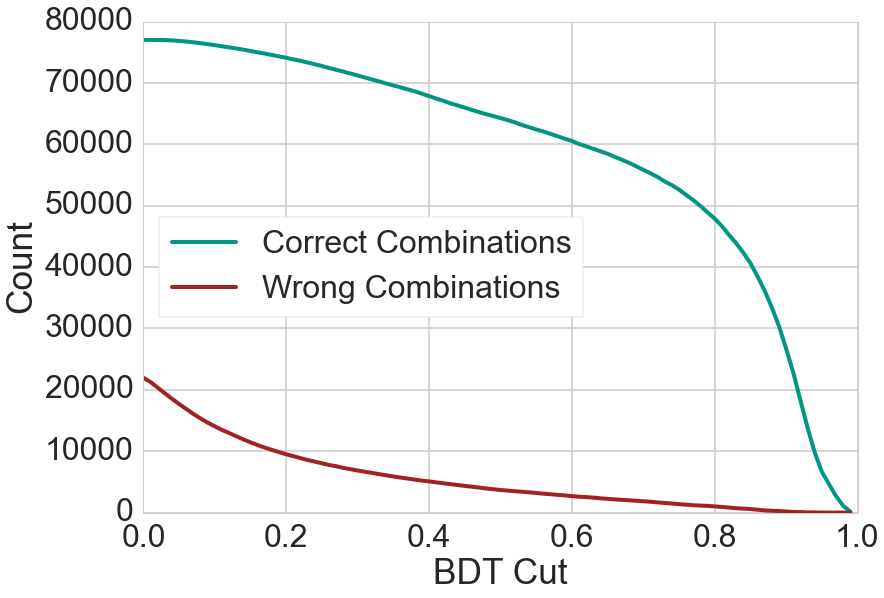
\includegraphics[width=0.7\linewidth]{figures/workflow/first_filter_count.png}
  \caption{Number of correct and wrong segment--track-combinations passing the BDT filter. As the pre-cut of at least one shared hit throws away much of the wrong combinations, the number of correct ones is larger from the start on.}
  \label{fig-first-filter-count}
  % Not comparable
  % Final
\end{figure}

\begin{figure}
  \centering
  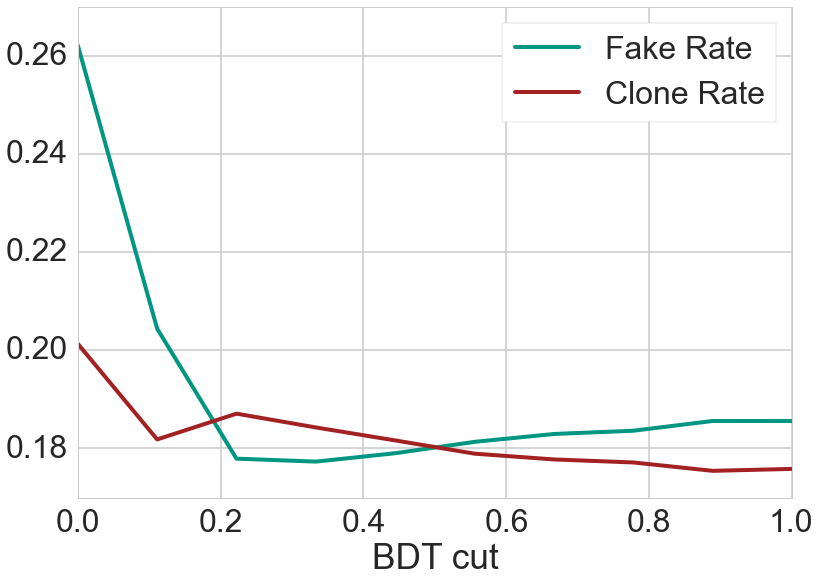
\includegraphics[width=0.48\linewidth]{figures/workflow/first_filter_rate.png}
  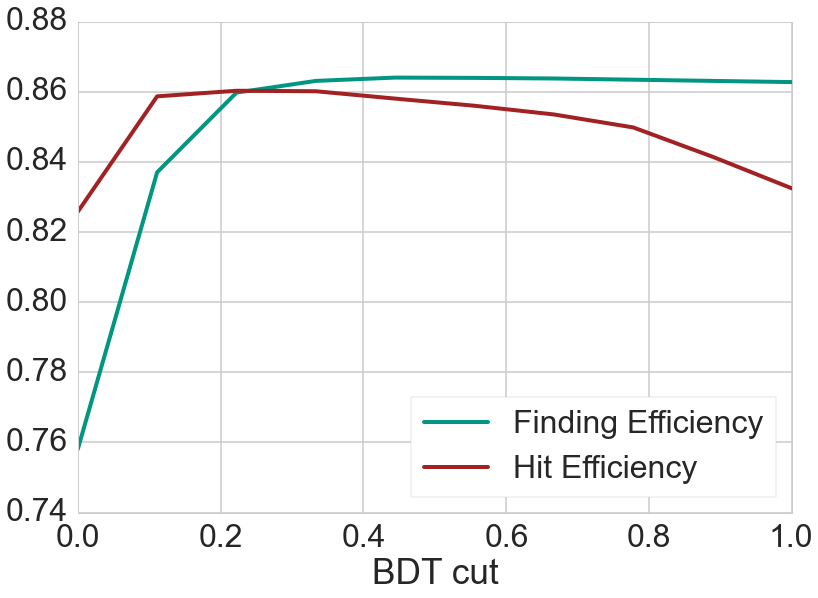
\includegraphics[width=0.48\linewidth]{figures/workflow/first_filter_efficiency.png}
  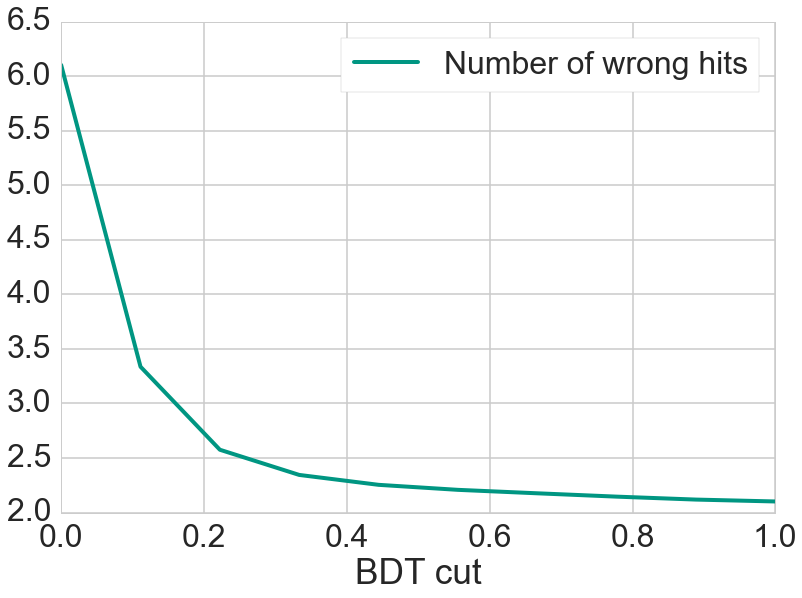
\includegraphics[width=0.48\linewidth]{figures/workflow/first_filter_wrong_hits.png}
  \caption{Figures if merit for different cut values on the BDT output of the first filter in the \texttt{SegmentTrackCombinerDevModule} with all other filters deactivated.}
  \label{fig-first-filter-fom}
  % On Input Data 2
  % Final
\end{figure}


% \paragraph{More complex matching (step \ref{list-fakes} and \ref{list-second})}
% The still remaining segment could either not be matched by the first matching procedure or do not share a hit with one of the tracks coming from the Legendre track finder. For these segments, an advanced matching routine is applied which starts by filtering out fake segments with a BDT using similar variables as the background hit finder. In the next step, the remaining segments are combined with the tracks. Beforehand, another filtering algorithm tries to combine the segments in one superlayer to larger segments, as the segment finder algorithm has problems with large segment especially in stereo layers. Both filters use typical segment properties like $p_T$ or the number of hits as well as high-level variables like the p-Value of a circular fit or distances between the segments or to the tracks. The filters however show a very bad performance and can not increase the hit efficiency without reducing the finding efficiency because a high number of fakes is produced. Therefore, these filters are not used in the following. \todo{???}

\paragraph{Filtering of the tracks (step \ref{list-end})}
To reduce the fake rate further before giving the tracks to the track fitter and the physics analysis packages, a trained BDT can filter out tracks that are most likely to be fakes. The BDT is trained using the fake flag output of the MC matching routine as the truth information. To classify whether a track is a fake, it uses several input variables compiled from the tracks trajectory and hit content as $p_T$ and $\tan \lambda$, a flag whether a segment could be matched to the track or the first two moments of the drift length or ADC count distributions among the hits. It also calculates a value to measure how ``empty'' the track is, i.e.\ how many hits are probably missing as a track with more missing hits is typically a fake. Figure~\ref{fig-track-filter-count} shows the output of the trained BDT. As it can be seen, the performance of the filter looks comparable to the other trained filters in this thesis. In this case however, every wrongly classified and deleted signal track reduces the finding efficiency directly. Figure~\ref{fig-track-filter-results} shows the figures of merit as a function of the BDT cut value on this filter only and confirms this conclusion as it has a high impact on the finding efficiency -- but also on the fake and the clone rate.
Higher cut values are unusable for the normal track finding path as the finding efficiency is reduced too much, however they can be used in situation where a very low fake rate and a high purity is necessary. In the following, a cut value of 0.1 is used.

\begin{figure}
  \centering
  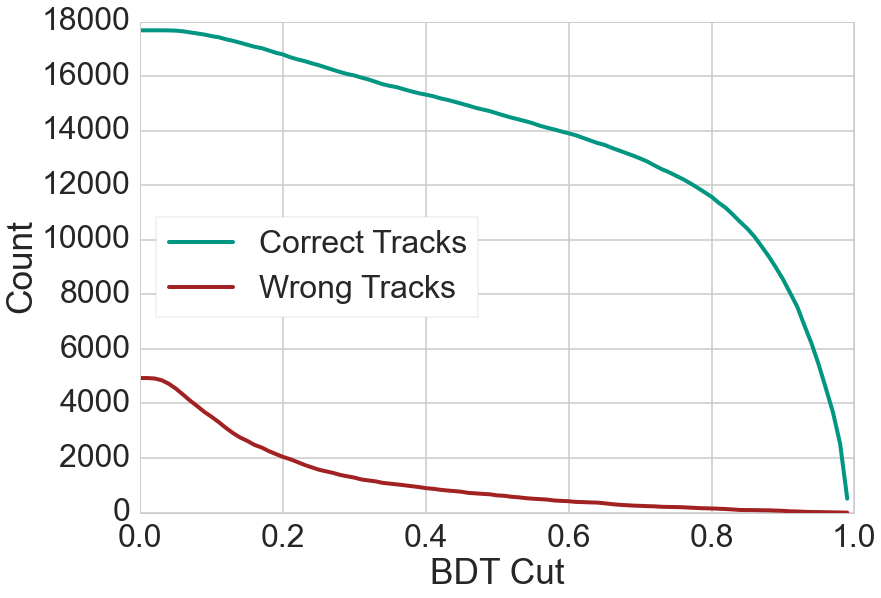
\includegraphics[width=0.7\linewidth]{figures/workflow/track_filter_count.png}
  \caption{Output of the track filter in the \texttt{SegmentTrackCombinerDevModule} in the last step which should separate fakes and signal tracks. The number of wrong tracks can be reduced with the BDT, however also the number of correct tracks is affected strongly.}
  \label{fig-track-filter-count}
  % Not comparable
  % On Input Data 2
  % Final
\end{figure}

\begin{figure}
  \centering
  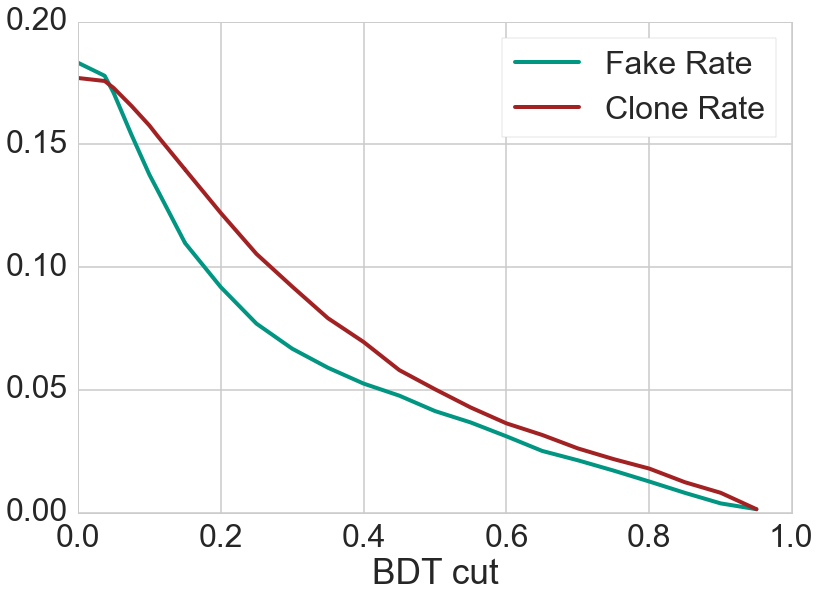
\includegraphics[width=0.48\linewidth]{figures/workflow/track_filter_rate.png}
  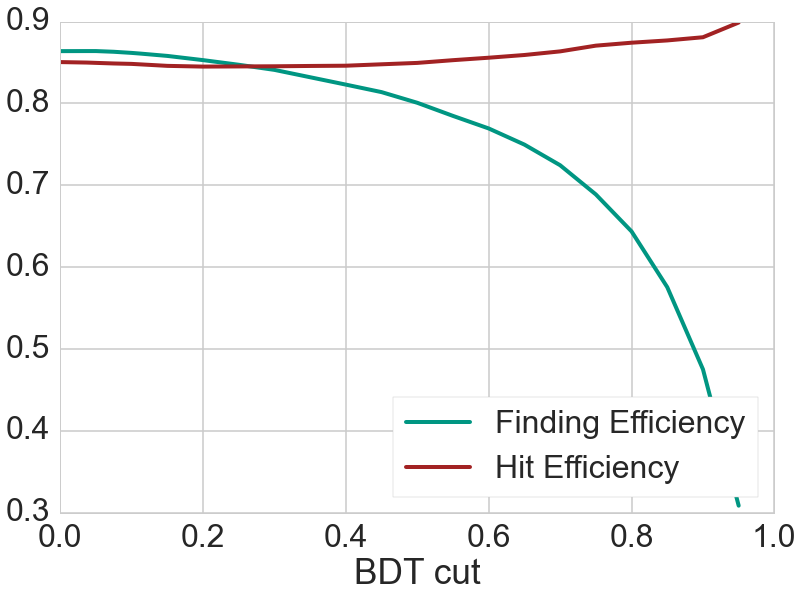
\includegraphics[width=0.48\linewidth]{figures/workflow/track_filter_efficiency.png}
  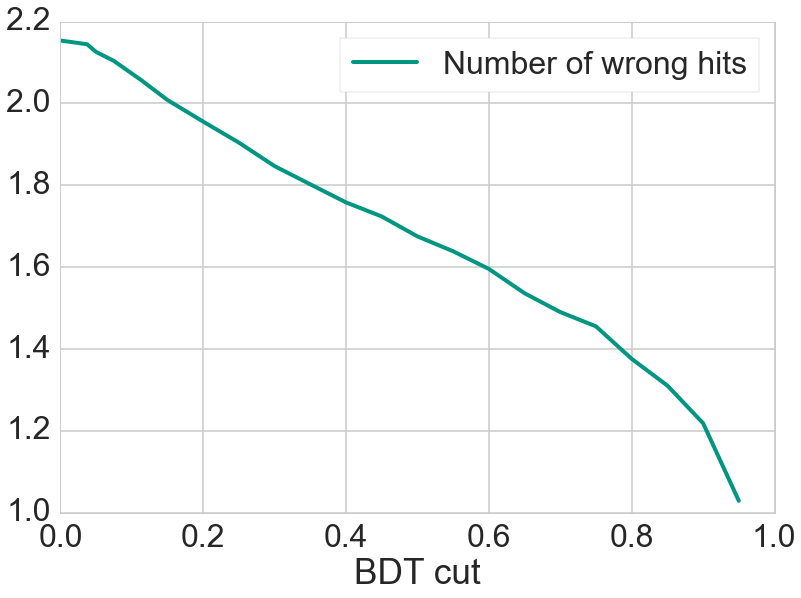
\includegraphics[width=0.48\linewidth]{figures/workflow/track_filter_wrong_hits.png}
  \caption{Results after the track filter in the \texttt{SegmentTrackCombinerDevModule}. As discussed in the text, the filter has a huge impact on the finding efficiency as well as the fake rate. Special demands for high-purity tracks may need higher cut values of such a filter in the future, while in the normal path only a small cut value is used.}
  \label{fig-track-filter-results}
  % On Input Data 2
  % Final
\end{figure}

\subsection{Results}

Table~\ref{tab-segment-track-combiner-fom} shows the figures of merit of the Legendre track finder (axial and stereo) also and after the combination with the segments from the local track finder. In the combination module, only the simple matching routine (step \ref{list-start}) is used. It can be seen that the finding efficiency stays on the same level whereas the hit efficiency could be increased. The fake rate is also reduced because of the implemented track filter (step \ref{list-end}). The other figures stay on the same level as before. The combination of the track finders is now superior over the reference implementation in nearly all aspects, except the number of wrong hits which can be reduced by applying certain quality tools described in the next section.

\begin{table}
  \caption{Table showing the figures of merit before and after the combination of Legendre track candidates with segments from the local track finder.}
  \centering
  \begin{tabular}{lccccc} \toprule
    & Legendre & Combination & Trasan & Old Implementation \\ \midrule
    Finding Efficiency   & 86.28 & 86.17 & 85.53 & 83.17 \\
    \quad on Primaries   & 92.32 & 92.19 & 91.49 & 89.94 \\ 
    Hit Efficiency       & 83.23 & 84.81 & 81.93 & 74.03 \\
    \quad on Primaries   & 88.96 & 90.60 & 87.25 & 78.22 \\ 
    Clone Rate           & 14.33 & 13.59 & 19.50 & 7.69 \\
    \quad on Primaries   & 7.63  & 7.02  & 17.17 & 4.71 \\ 
    Fake Rate            & 18.60 & 13.77 & 15.95 & 26.82 \\ 
    Wrong Hits per Track & 2.10  & 2.07  & 1.09  & 2.69 \\ 
    Time per Event in ms & 36.54 & 39.42 & 419.50& 635.05 \\ \bottomrule
  \end{tabular}
  \label{tab-segment-track-combiner-fom}
  % On InputData 2
  % Final
\end{table}

The still remaining segments of the local track finder can be classified uniquely into one of the four categories:
\begin{description}
  \item[Background] segments consist mainly of background hits,
  \item[Ghost] segments include more than one MC track candidate and it is not possible to relate them unambiguously to one MC particle\footnote{In contrast to the matching routine described in chapter~\ref{chapter-theory}, the both categories ``background'' and ``ghost'' are split up here, that were summarized in the ``fake'' category earlier.},
  \item[Segments with matching track] are neither fake nor background and share hits with a track from the Legendre algorithm and
  \item[Segments with no matching track] are also neither fake nor background and the related MC particle was not found by the Legendre track finder (or it is found but the Legendre track is tagged as a fake track).
\end{description}

The first two categories can be summarized into a ``Unmatchable'' category. Figure~\ref{fig-remaining-segments-full} shows the number of classified segments (left) and a detailed view with the ``Unmatchable'' category dissolved and without the segments with a matching track for better visibility (right). The numbers are shown before the combination with the Legendre tracks, after deleting all segments that share all hits with an unique Legendre track, after the first matching step (step~\ref{list-start}), and after deleting probably ghost or background segments (step~\label{list-fakes}). Before the combiner, most of the segments can be matched to a Legendre track, because the local track finder uses the same (full) hit set as the Legendre track finder and finds most of the times the same tracks and hits. Deletion of all segments that share all hits with a Legendre track and can therefore not improve any figure of merit as they do not add any new information leads to a strong reduction of the total number of segments mainly because the number of segments with a matching track was decreased. Theoretically, there is no need to find those segments again by the local track finder after the Legendre track finder, but it is not inherently clear which hits of the whole event after the Legendre track finder should not be used by the automaton track finder and which of them are needed to add additional information to the tracks.\footnote{The problem is, that because of the principle of operation of the local track finder, it can only find segments if the hits of the full neighborhood -- even better the whole segment -- are used as input to the algorithm. So not using all hits that are already used by the Legendre track finder would lead to no found segments at all. Not even the ones belonging to new tracks because the Legendre track finder has probably used parts of those hits in fake tracks.} The number of ghost and background segments is not changed due to this deletion. However, the number of segments with no matching track is reduced as well due to the fact, that some of those segments were classified in this category because they only share hits with a fake Legendre track and are now as well deleted. The first matching step (step~\ref{list-start}) reduces the number of segments with a matching track again by more than a factor of two while not changing the other numbers (except the tracks with no matching tracks slightly for the same reason as before), which shows that the implemented algorithm works well. As can also be seen, the following filter to delete background segments, which is not described here, does effectively reduce the number of background segments while keeping all other numbers steady. In the end, the remaining segments consist approximately of 50 \% segments with matching track, 17 \% describing new tracks, 10.3 \% background segments and 22.7 \% ghost segments. The total number of segments however was reduced to about 16 \% of their initial size. Still, there is further development needed to reduce the number of segments with a matching track to use the remaining segments to find new tracks.

\begin{figure}
  \centering
  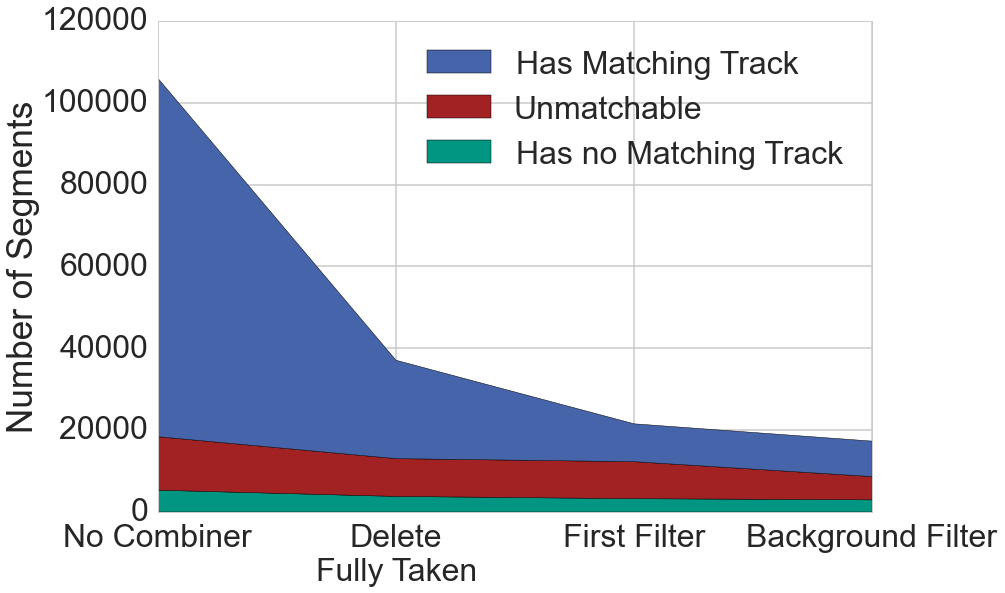
\includegraphics[width=0.48\linewidth]{figures/workflow/remaining_segments_full.png}
  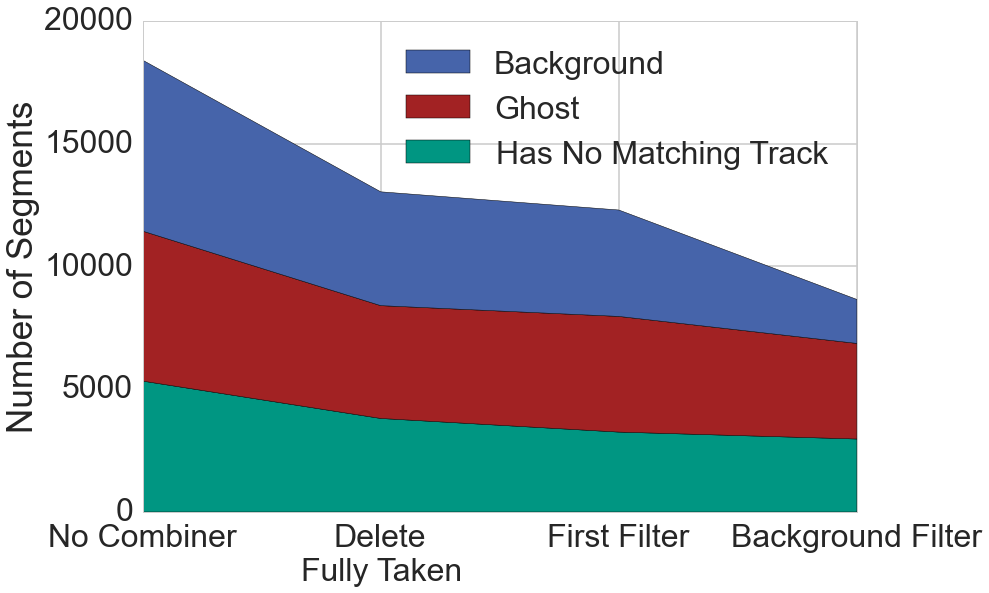
\includegraphics[width=0.48\linewidth]{figures/workflow/remaining_segments_detail.png}
  \caption{Number of segments in the four categories in a stack plot after various steps in the combiner module as described in the text. In the left figure the background and ghost category are merged into ``Unmatchable'', whereas in the right plot the segments with matching Legendre tracks are not shown. The effect of the filter steps can be seen clearly.}
  \label{fig-remaining-segments-full}
  % On Input Data 2
  % Not comparable
  % Final
\end{figure}


\section{The \texttt{Track\-Quality\-Asserter\-CDC\-Module} and the \texttt{Track\-Quality\-Tools}}  \label{section-quality}

The common code basis in the CDC track finding package makes it possible to include common correction tools for the resulting tracks into the software framework. The \texttt{TrackQualityTools} singleton offers functions for applying typical corrections on the track candidates like removing of hits or normalizing the trajectory information to a defined format (e.g.\ the start point of the circular trajectory should lay on the position of the first hit). The different implemented methods are described later.

These tools can be used in the track finder modules directly (instead of implementing the same algorithms again), but can also be used standalone (with the module \texttt{TrackQualityAsserterCDC}) after the whole track finding procedure. The reason is not only to reduce the number of wrong hits per track and the fake rate, but also to prepare the tracks for the next step, the track fitting. The fitting algorithm needs a defined format for the trajectory seed parameters (the position seed must lay near the first hit in the track and the momentum seed must be defined at this point). Additionally, the fitting algorithm as it is currently implemented in the framework is very sensible to inconsistencies in the track candidates like long sections of missing hits or wrongly added hits because of decay-in-flight particles or high energy loss. The fit can get biased into a wrong direction in the first iteration leading to an increased number of total iteration steps and a higher computing time because of more needed material lookups. As the maximal number of iteration per track is limited to improve performance, the fit can fail completely reducing the finding efficiency when taking into account only fitted tracks to about 82 \% (compared to the values of about 92 \% before the fit for primaries). To increase the number of successful fits, the tracks can be edited to be suited for fitting including the clipping of hits. As only the tracking parameters at the front of the track are important for physics analysis, cutting away parts of the track does not harm the fit resolution directly. The hits however can be used in $\mathrm d E/\mathrm d x$ analysis for particle identification and it may be a good idea to keep the relation to the track and readd them to the fitted results to increase the hit efficiency again. 

Another important step is the removal of axial only tracks which can not be fitted by the currently implemented track fitting procedures as there is no direct $z$ information present in the tracks.\footnote{Tracks without stereo hits have nevertheless a $z$ information in them as the energy loss depends in the travel length in the material which in turn is related to the $\theta$ angle of the track. \cite{martin}} As most of these tracks have no stereo hits because the energy is too low to reach into the first stereo superlayer and not because the track finder algorithms have not found the hits, there is no possibility to add stereo information to the tracks in the CDC only. A different approach -- combining the CDC track candidates with the VXD results -- is shown in section~\ref{section-outlook}.

When only taking into account fitted tracks, the finding efficiency could be increased with running the \texttt{Track\-Quality\-Asserter\-CDC} module before fitting, but does not reach the finding efficiency before the fit -- so the fitting rate is not 100 \% still -- and also not the one from trasan. The finding and hit efficiency together with the other figures of merit are shown in table~\ref{tab-results-after-fitting} before and after the fit with and without the quality module. As can be seen, the number of wrong hits per track could be reduced by the quality corrections - also the fake rate is improved drastically. The computing time of the fitting module could be reduced from $\unit[1600]{ms}$ per event (which is much too large) to around $\unit[680]{ms}$. In figure~\ref{fig-efficiency-after-fitting} the finding efficiency over $p_T$ is shown before and after the fit (without and with the quality tools). It can be seen that the corrections can increase the rate of fitted tracks especially in the low-momentum region, but the fit still fails especially for these curling tracks. Once the external fitting package is improved to handle these challenging cases also, some of the corrections can be turned off by changing the steering file parameters of the module.

\begin{table}
  \caption{Figures of merit with and without the track quality asserter module in the end of the path before the fit and with the not-fitted tracks removed. For comparison, the reference implementation trasan is also shown.}
  \centering
  \begin{tabular}{lcccccc} \toprule
    & \multicolumn{3}{c}{Before Fitting} & \multicolumn{3}{c}{After Fitting} \\ 
    & No Quality & Quality & Trasan & No Quality & Quality & Trasan \\ \midrule
    Finding Efficiency   & 86.17 & 85.16 & 85.53 & 73.75 & 77.69 & 82.30 \\
    \quad on Primaries   & 92.19 & 91.24 & 91.49 & 82.40 & 86.44 & 89.83 \\ 
    Hit Efficiency       & 84.81 & 83.30 & 81.93 & 85.57 & 84.69 & 82.71 \\
    \quad on Primaries   & 90.60 & 89.11 & 87.25 & 90.45 & 89.32 & 87.30 \\ 
    Clone Rate           & 13.59 & 11.60 & 19.50 & 3.67  & 3.77  & 14.56 \\
    \quad on Primaries   & 7.02  & 5.45  & 17.17 & 2.70  & 2.83  & 12.75 \\ 
    Fake Rate            & 13.77 & 8.02  & 15.95 & 3.48  & 2.74  & 3.44 \\ 
    Wrong Hits per Track & 2.07  & 1.70  & 1.09  & 1.75  & 1.47  & 0.91 \\
    Time per Event in ms & 39.42 & 42.53 & 419.50& 1079.37 & 668.15 & 571.23 \\ \bottomrule
  \end{tabular}  
  \label{tab-results-after-fitting}
  % On InputData 2
  % Final
\end{table}

\begin{figure}
  \centering
  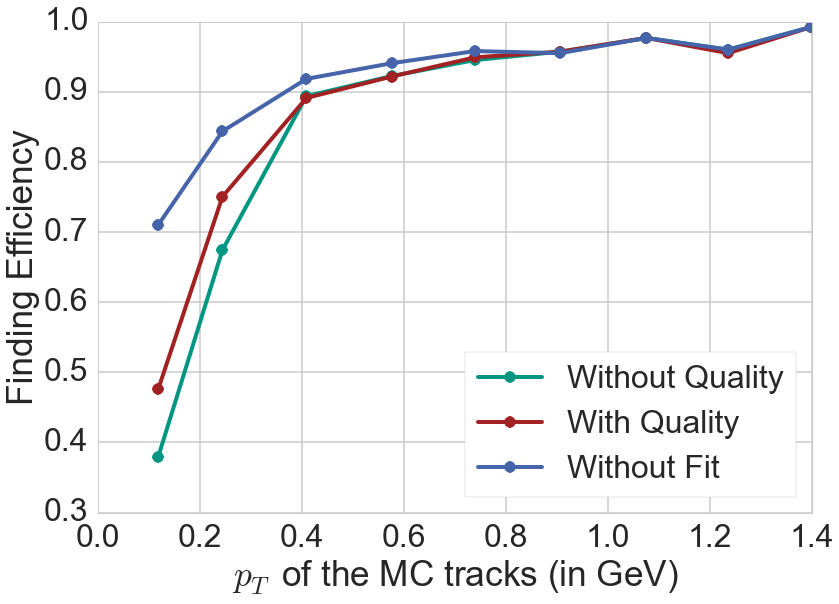
\includegraphics[width=0.7\linewidth]{figures/workflow/efficiency_after_fit.png}
  \caption{Finding efficiency over $p_T$ for the full path with and without the quality corrections applied after removing all not-fitted tracks. For comparison, also the efficiency before the fit and without the quality tools is shown in blue.}
  \label{fig-efficiency-after-fitting}
  % On InputData 2
  % Final
\end{figure}

Some of the methods implemented in the \texttt{TrackQualityTools} are described with more details in the following:
\begin{description}
 \item[\texttt{normalizeHitsAndResetTrajectory}] To have a defined starting point in each of the modules and especially for the fitting routines, the trajectory is shifted to start near the first track hit. This hit is determined to be the most inner hit of the track and has an arc length\footnote{The arc length is calculated by assuming a circular shape of the trajectory} of zero by definition. All other hits have positive arc lengths and are sorted according to these values. The trajectory for curling tracks is reversed for that the number of hits on the ingoing arm is greater than on the outgoing one.
 \item[\texttt{removeHitsAfterLayerBreak} and \texttt{removeArcLength2DHoles}]  As the fitting procedure can not handle tracks with large sections of not found hits very well, it is feasible to have routines which cut tracks before those holes. This can be done either by looking on the arc length or the geometrical distance between successive hits in the tracks. An additional method can cope with multiple ``breaks'' in the track and chooses the longest coherent track part.
 \item[\texttt{removeHitsOnTheWrongSide}] The Legendre track finding algorithm has some issues with non-curling back-to-back tracks or at least hits. The problem can be seen in figure~\ref{fig-b2btrack}. For non-curling tracks these added hits can easily be spotted by looking onto the arc length values which is negative for these hits.
 \item[\texttt{splitSecondHalfOfTrack}] As the reference implementation trasan, which was used successfully in combination with the fitting algorithms currently implemented, splits every curling track on the apogee point, this feature is also implemented in the track quality tools.
\end{description}
In addition, there are methods to remove tracks with a small number of hits or which are localized in a single super layer and other methods which are not described here. Picture~\ref{fig-quality} shows a event display before and after some of the quality corrections in the module. As can be seen in the figure, most of the wrong hits of the tracks are deleted after the quality improvements. In the full path presented in this thesis, the quality tools to remove hits on the wrong side, to remove tracks in only one superlayer or with a small number of hits, and to reduce the number of large breaks in a track are used.

\begin{figure}
  \centering
  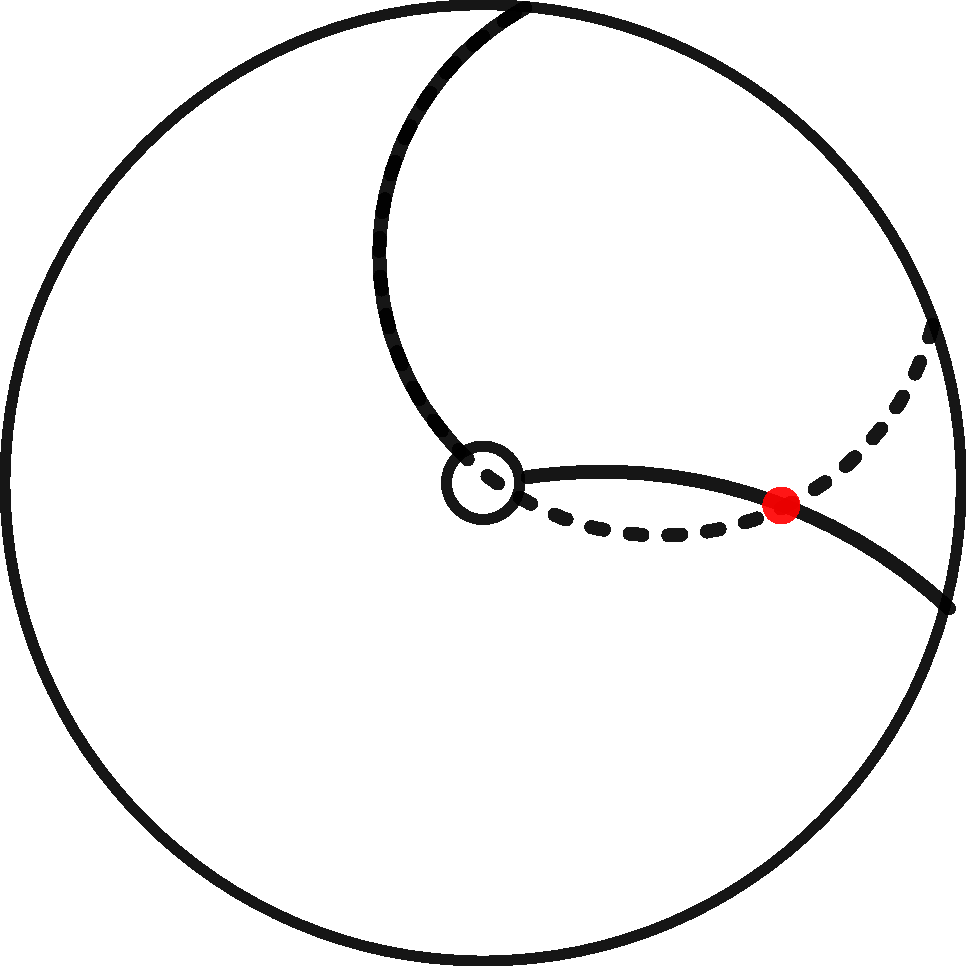
\includegraphics[width=0.48\linewidth]{figures/workflow/B2B.pdf}
  \caption{Picture showing the problem with hits on the wrong side of the track. The red hit gets added to the left track incorrectly, as the extrapolation (dashed line) through the interaction point leads to an intersection with the hit although it should belong to the right track. This problem is rather easy to solve by looking onto the arc length of the hits.}
  \label{fig-b2btrack}
  % Final
\end{figure}

\begin{figure}
  \centering
  \begin{tikzpicture}[>=latex']
    \def\x{4}
    \def\y{4}
    \node at (1.5*\x + 1, 11) {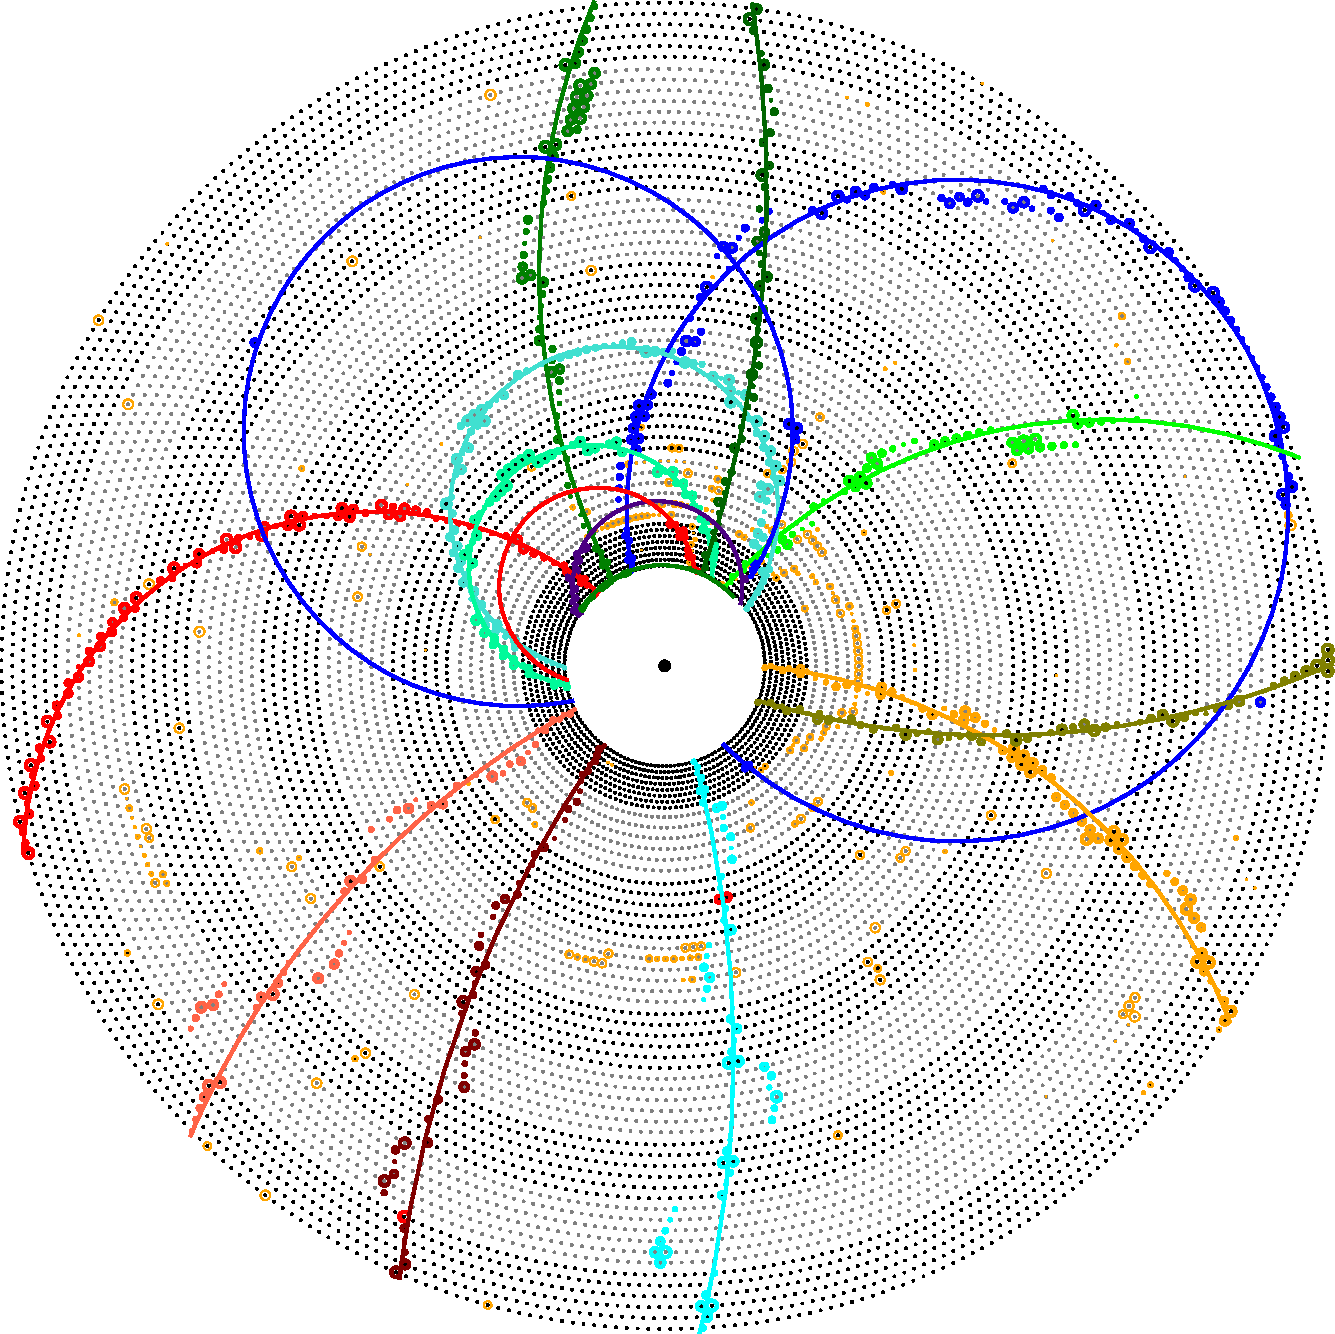
\includegraphics[width=0.8\linewidth]{figures/workflow/before_quality.pdf}};
    
    \draw[black, rounded corners, fill=white] (0, 0) rectangle (\x, \y);
    \draw[black, rounded corners, fill=white] (\x + 1, 0) rectangle (2*\x + 1, \y);
    \draw[black, rounded corners, fill=white] (2*\x + 2, 0) rectangle (3*\x + 2, \y);
    
    \node[anchor=south west, inner sep=0] at (0.1, 0.1) {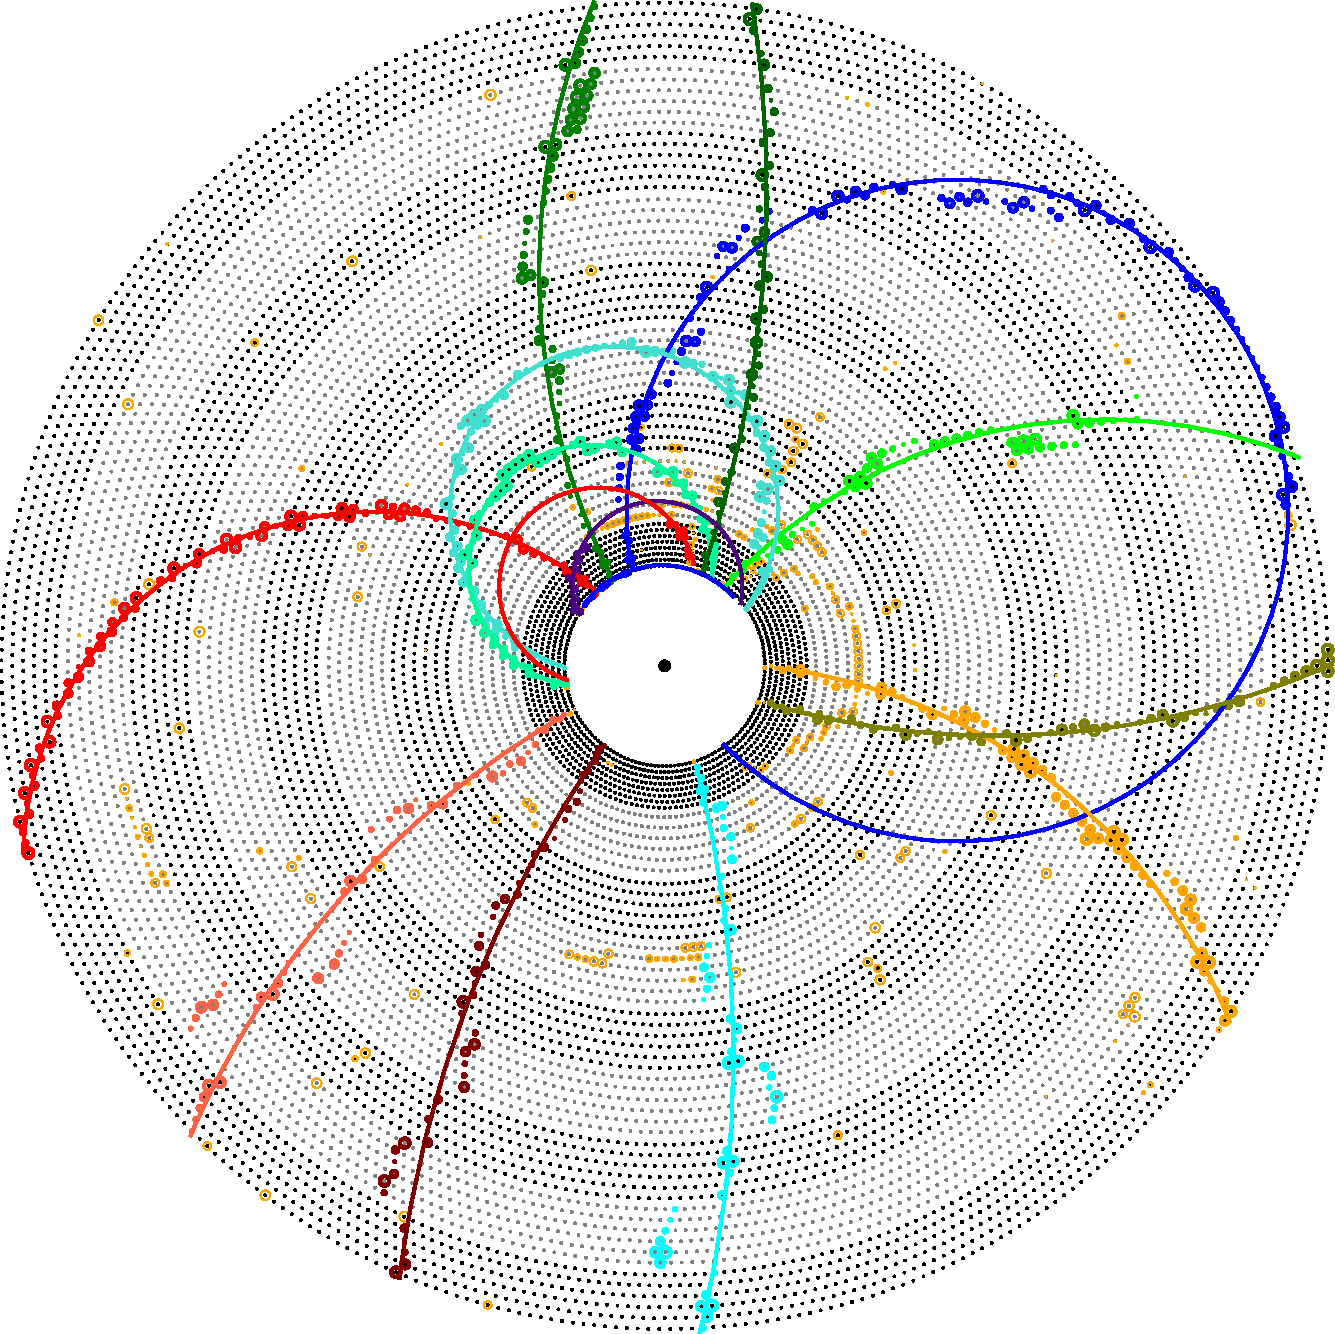
\includegraphics[trim={4.5cm 10.2cm 8.6cm 2.9cm}, clip, scale=0.4]{figures/workflow/after_quality.pdf}};
    \node[anchor=south west, inner sep=0] at (5.1, 0.1) {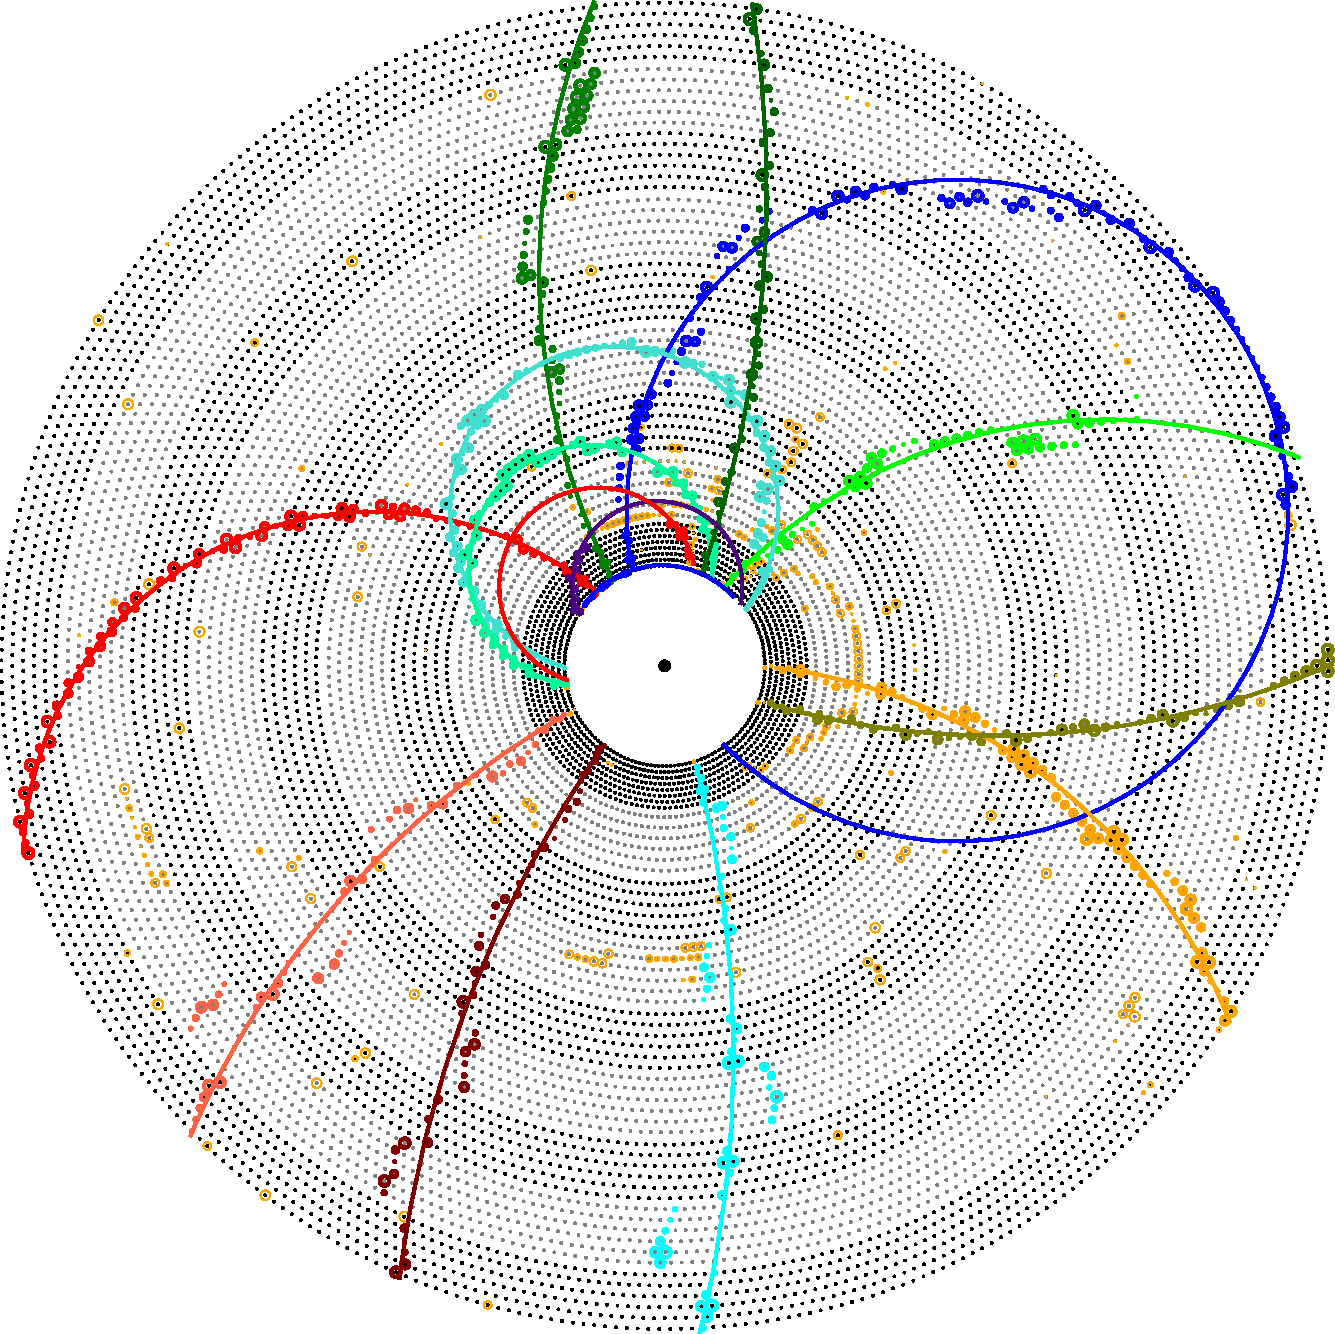
\includegraphics[trim={10cm 5cm 8.8cm 13.8cm}, clip, scale=1]{figures/workflow/after_quality.pdf}};
    \node[anchor=south west, inner sep=0] at (10.1, 0.1) {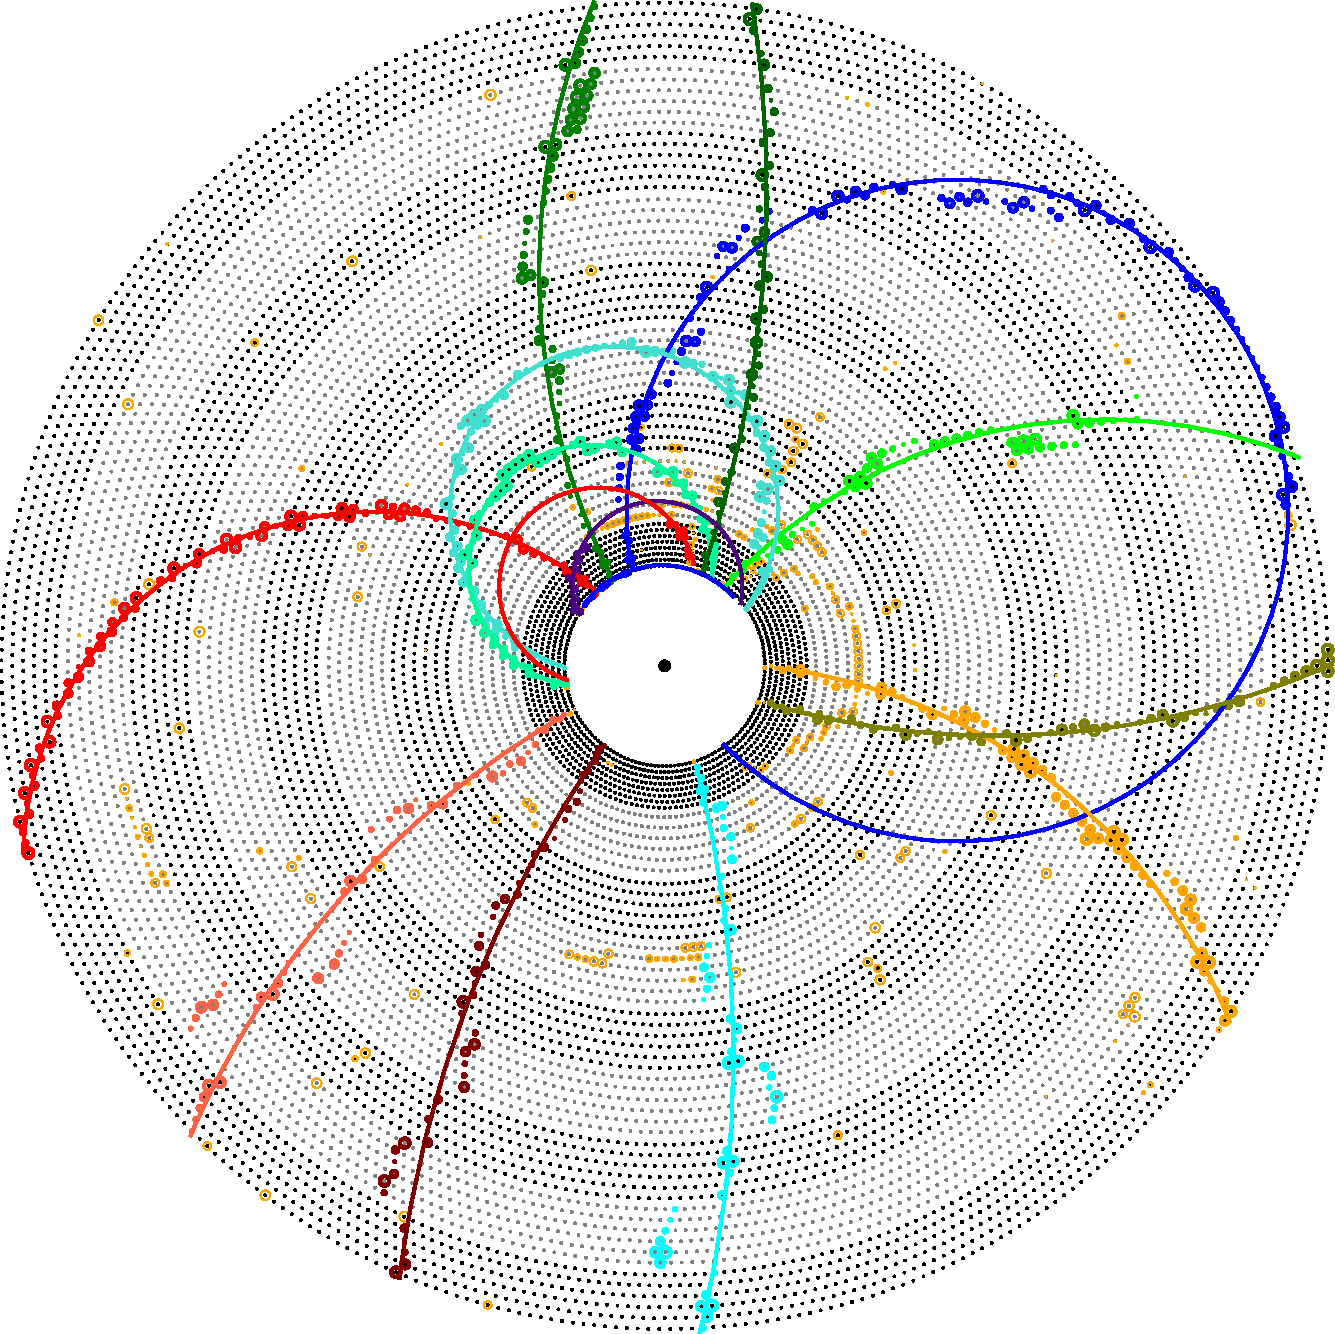
\includegraphics[trim={10.5cm 7.2cm 8.3cm 11.6cm}, clip, scale=1]{figures/workflow/after_quality.pdf}};

    \draw[kit-red100,ultra thick,rounded corners] (6.8, 2) rectangle (7.8, 3);
    \draw[kit-red100,ultra thick,rounded corners] (11.8, 2) rectangle (12.8, 3);
        
    \draw[->, thick] (0.5*\x, \y) -- (3.65, 11);
    \draw[->, thick] (2*\x + 0.5, \y) -- (7.65, 8.5);
    \draw[->, thick] (3*\x, \y) -- (7.85, 9.75);
    
  \end{tikzpicture}
  \caption{Event display before (top) and after (below, cut-offs) the quality corrections. The orange fine circles indicate hits that are not attached to a track. The cut-offs show the locations where the quality improvements have deleted whole tracks (the blue one in the first picture) or wrong hits (second and last picture).}
  \label{fig-quality}
  % Calculated using InputData2 and not comparable to the rest! (but can also not compared)
  % Final
\end{figure}

\section{Further Approaches} \label{section-outlook}

Besides the presented workflow shown in figure~\ref{fig-workflow2}, there are of course other ways to combine the outputs of the two track finders and prepare the tracks for the fitting procedure and the physics analyses. The most promising, the axial quad tree search with segments instead of hits analogous to the stereo finder with segments, is presented first. Then, the problem of connecting the results of both the CDC and the two VXD detectors is discussed. Both methods were not implemented fully during this thesis and can be optimized further.

Besides implementing new algorithms with different approaches, also the already discussed workflow can be further refined and optimized. Possible optimization steps include the addition of other coordinate axes to the quad tree search algorithms (to cope for example with large energy loss of the particles or to combine the axial and the stereo finder in one search), cross-detector uses of the algorithms (by applying the quad tree search for CDC and VXD hits in parallel \cite{markus}) or further boost of the computational performance (e.g.\ by using parallelization or GPUs).

\subsection{Quad tree search with segments}

As seen in section~\ref{section-fom}, the huge benefit of segments is their high purity. Using segments instead of hits in the Legendre quad tree search has various advantages like the reduced combinatorics making more coordinate axis in the Legendre space possible\footnote{Possible candidates for this new coordinate axis are $\tan \lambda$ to combine axial and stereo segments at the same time or a coordinate to include energy loss.} or the reduced needs for post-processing after the track finding as a hit-reassignment is often unneeded. Also, the segments from the automaton track finder already include a left--right-information which reduces the number of sinograms in the Legendre space by a factor of two. However, one has to think about the way the decision is made whether a segment belongs to a quad tree bin or not. There are several possibilities, e.g.\ using the averaged position of the included hits with the same algorithm as with single hits, checking all hits independently and use the segment only of more than a certain percentage lay in the quad tree bin, use facets instead of single hits, include the direction information of the segments, etc. Some of them are shown in the following.

Figure~\ref{fig-quad-tree-segments} shows the Legendre space of a simplified event (refer to figure~\ref{fig-quad-tree-event} for an event display) with the positions of the segments shown as points colored by their MC particle information. The whole segment has already trajectory parameters computed by a circular fit attached to it, so the segment is a single point in the Legendre space rather than a sinogram. As can be seen in the figure, the segment points for one MC track do not meet in one single point but are rather spread around a whole Legendre space region also mixing different particles. The reason for this is, that the trajectory information is created using only the small number of hits the segment has. As the lever arm is small, the trajectory parameters are often inaccurate. 

Figure~\ref{fig-quad-tree-averaged-hits} shows the same event as in figure~\ref{fig-quad-tree-event}, but this time using another way to transform the segments to the Legendre space: the hit positions in each segment are averaged and this averaged position is turned into a sinogram according to the usual function. Figure~\ref{fig-quad-tree-normal-hits} shows the normal sinograms using each hit separately as comparison. It is clearly visible that using the averaged position instead of all hits reduces the combinatorics and therefore the computation time drastically but keeps all the information necessary for finding track candidates.

The last possibility presented here can be seen in figure~\ref{fig-quad-tree-piece}: Each hit is treated separately, but a piece of the sinogram is only accepted if all hits in a segment lay in the same region (as this is done in discrete bins, the figure looks fragmented). Here also, the additional information of the segment can lead to lower combinatorics and more precise results, as the probability to include hits of other tracks is reduced.

\begin{figure}
  \centering
  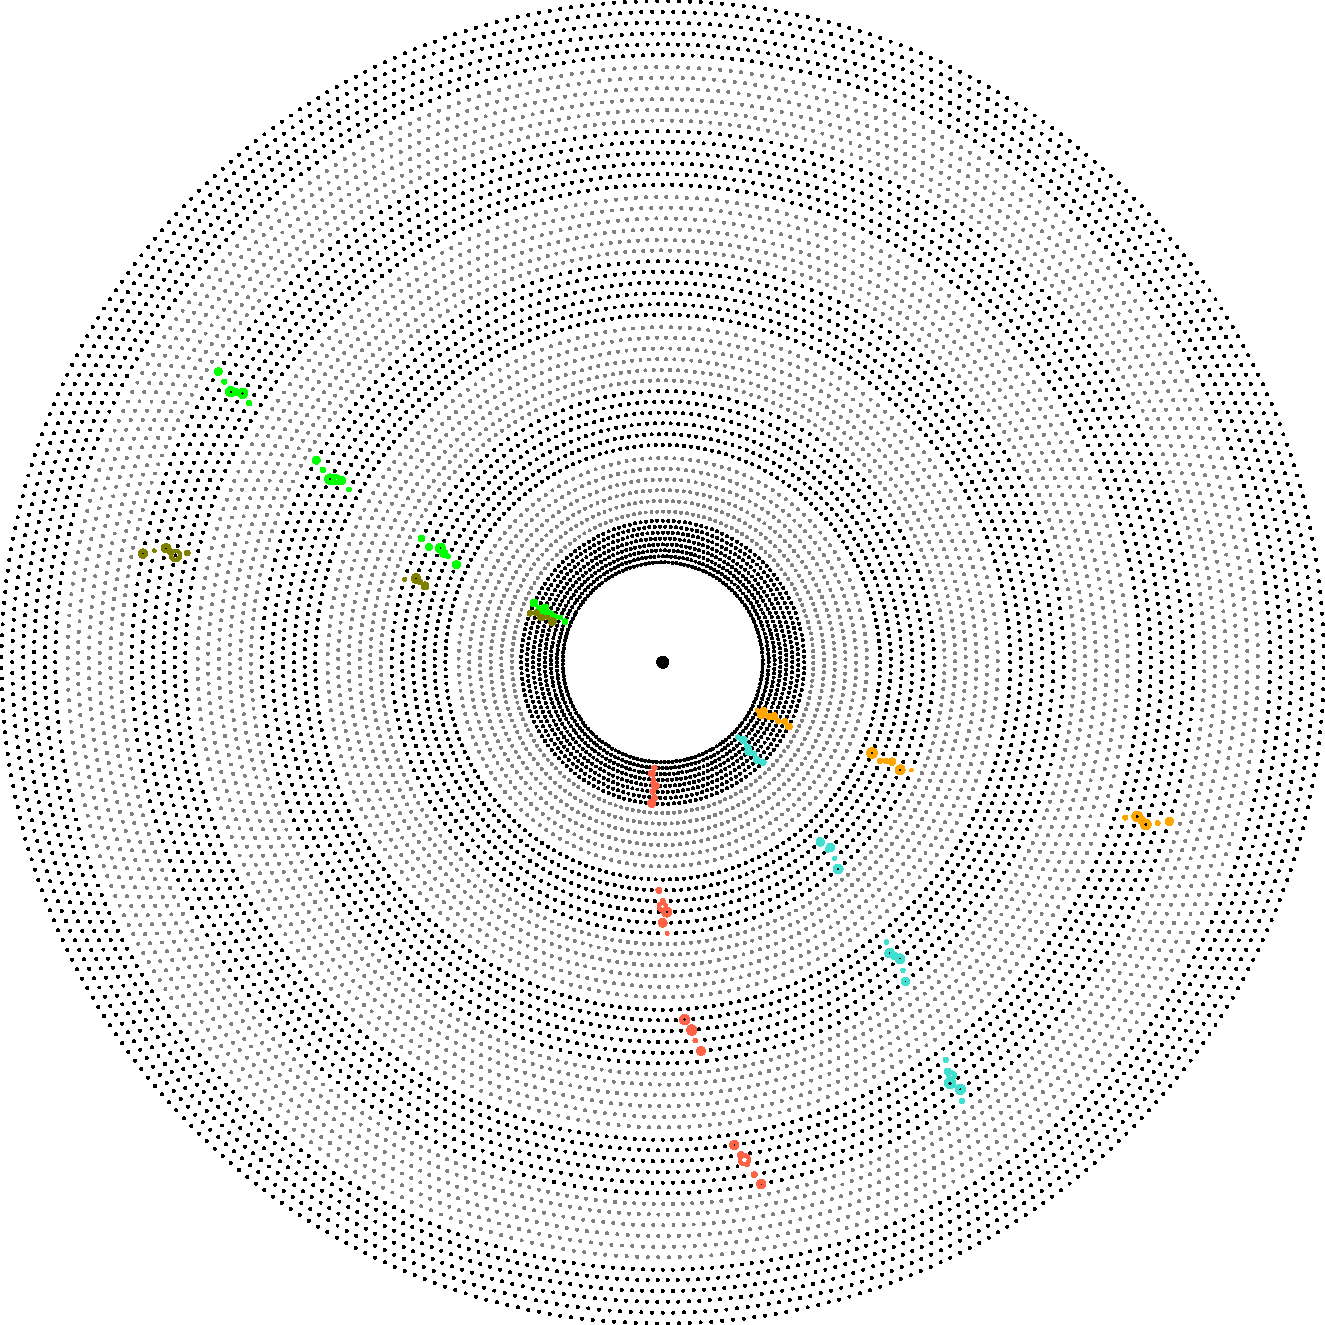
\includegraphics[width=0.9\linewidth]{figures/workflow/quad_tree_segments_event.pdf}
  \caption{Simplified event for visualizing the segment quad tree with the used segments colored with MC information. Note that not all segments are used in the picture to increase readability in the Legendre space plots.}
  \label{fig-quad-tree-event}
  % Calculated using simpliefied events and not comparable to the rest! (but can also not compared)
  % Final
\end{figure}

\begin{figure}
  \centering
  \begin{subfigure}[t]{0.48\linewidth}
    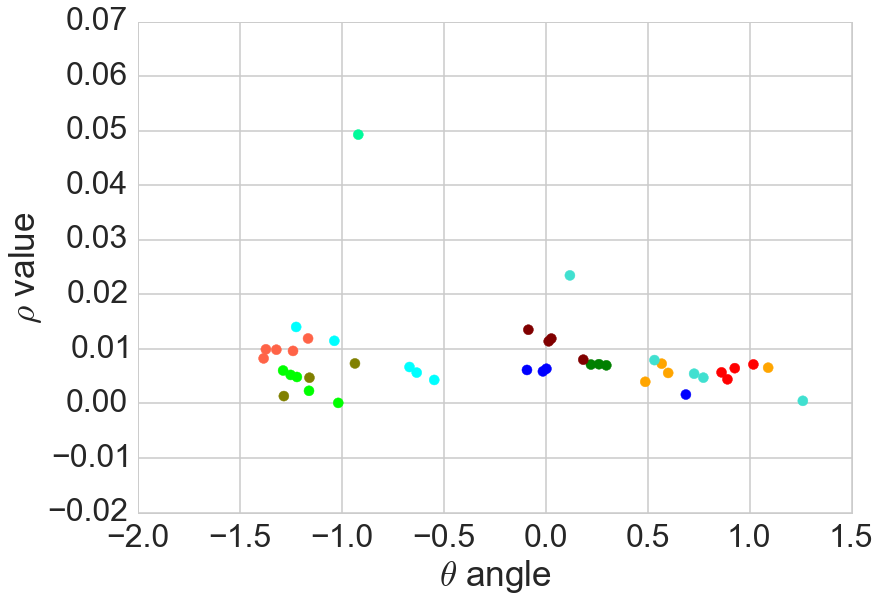
\includegraphics[width=\linewidth]{figures/workflow/quad_tree_segments.png}
    \caption{With segment parameters.}
    \label{fig-quad-tree-segments}
  \end{subfigure}
  \begin{subfigure}[t]{0.48\linewidth}
    \centering
    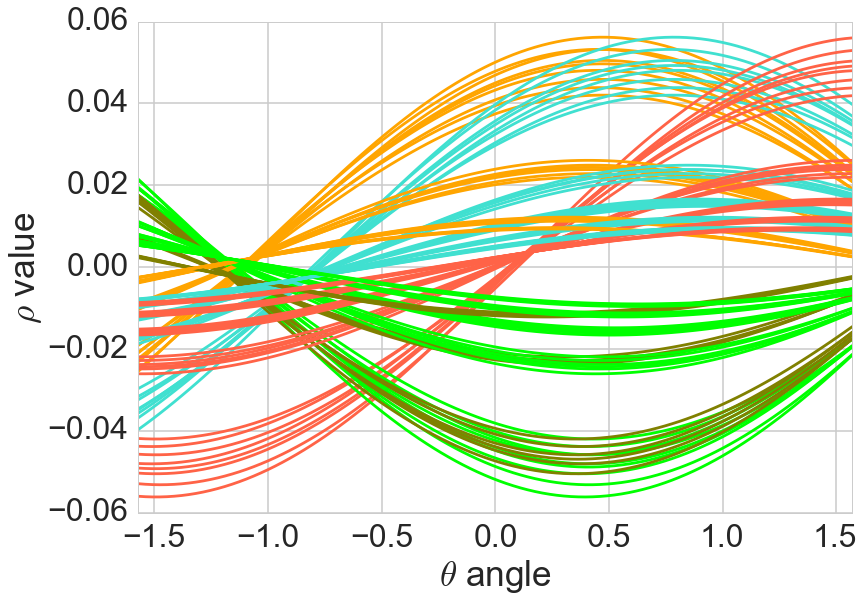
\includegraphics[width=\linewidth]{figures/workflow/quad_tree_normal_hits.png}
    \caption{With each hit separately.}
    \label{fig-quad-tree-normal-hits}
  \end{subfigure}
  
  \begin{subfigure}[t]{0.48\linewidth}
    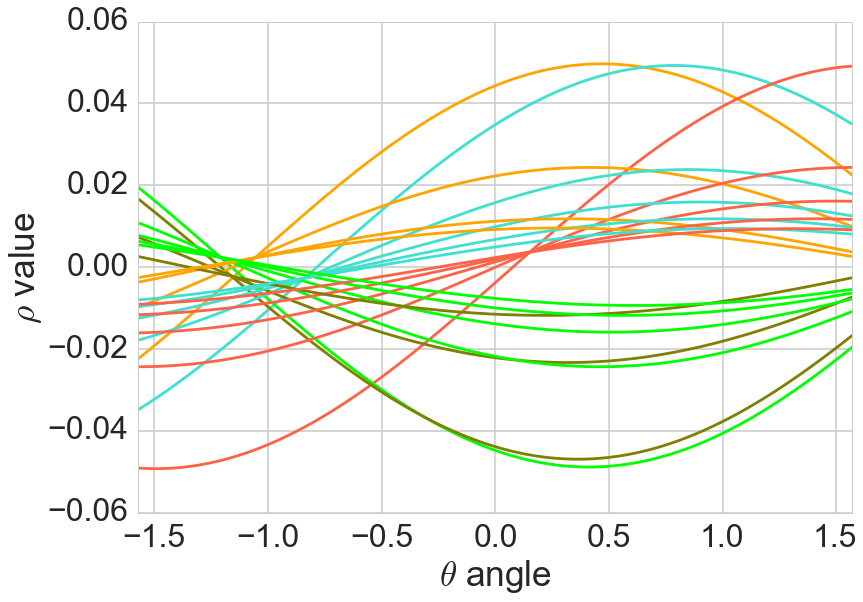
\includegraphics[width=\linewidth]{figures/workflow/quad_tree_averaged_hits.png}
    \caption{With the hits in each segment averaged.}
    \label{fig-quad-tree-averaged-hits}
  \end{subfigure}
  \begin{subfigure}[t]{0.48\linewidth}
    \centering
    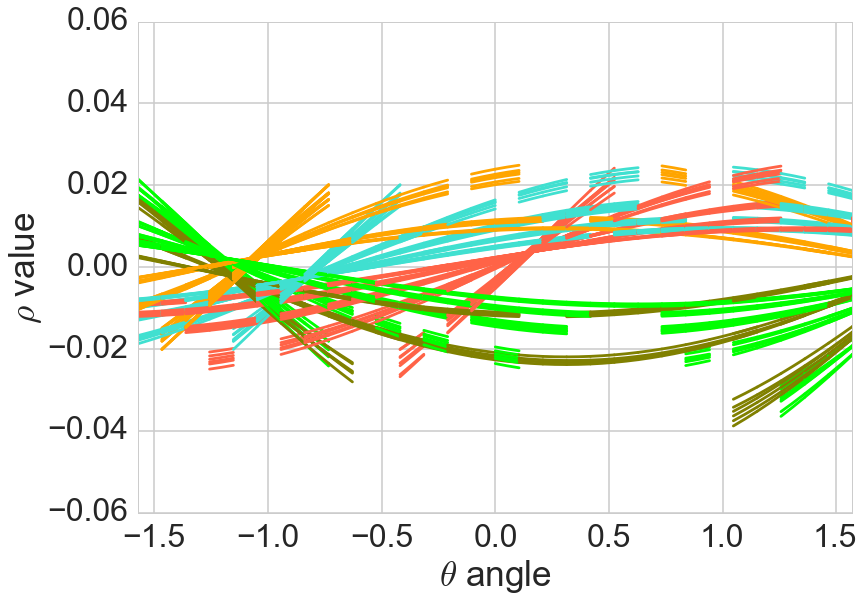
\includegraphics[width=\linewidth]{figures/workflow/quad_tree_piecewise.png}  
    \caption{With each hit separately, but checked if hits of a segment belong to the same region.}
    \label{fig-quad-tree-piece}
  \end{subfigure}
  
  \caption{Legendre space for some of the different possibilities to include the segment information in building the sinograms of the hits as described in the text. The color code is the same as shown in figure~\ref{fig-quad-tree-event}.}
  % Calculated using simpliefied events and not comparable to the rest! (but can also not compared)
  % Final
\end{figure}

Table~\ref{tab-quad-tree-segments} shows the figures of merit for the presented quad trees with segments and the axial Legendre track finder as described in the sections before. It can be seen, that the figures for the new segment quad trees are clearly worse than the ones for the Legendre track finder, but in view of all the post-processing and merging procedures implemented in this module that are still missing in the new quad trees with segments, the results are promising.

\begin{table}
  \caption{Figures of merit of the quad tree implementations with segments (for axial hits only) in comparison to the axial Legendre track finder. As expected, the quad trees with segments perform worse.}
  \begin{tabular}{lcccc} \toprule
    & Axial Legendre & Parameters & Averaged Position & Region Check \\ \midrule
    Finding Efficiency   & 86.84 & 48.47 & 35.49 & 60.12 \\
    \quad on Primaries   & 93.20 & 52.45 & 39.34 & 65.98 \\ 
    Hit Efficiency       & 48.52 & 25.24 & 37.60 & 40.13 \\
    \quad on Primaries   & 51.48 & 25.47 & 38.54 & 41.21 \\ 
    Clone Rate           & 13.33 & 15.43 & 9.06  & 11.32 \\
    \quad on Primaries   & 7.67  & 17.24 & 15.50 & 11.11 \\ 
    Fake Rate            & 19.09 & 14.43 & 52.10 & 26.03 \\ 
    Wrong Hits per Track & 1.08  & 1.17  & 8.23  & 3.97 \\ 
    Time per Event in ms & 36.07 & 16.68 & 20.94 & 42.64\footnotemark \\ \bottomrule
  \end{tabular}
  \label{tab-quad-tree-segments}
  % Calculated using InputData 7 and not comparable to the rest! (but can also not compared)
  % Final
\end{table}

\footnotetext{As the other approaches, especially this implementation uses a non-optimal algorithm to add the hits of the segments to a quad tree bin and the computation time can be increased further.}

\subsection{VXD-CDC-Merger before fitting}
In the steps following the track fit with the genfit package, the found and fitted CDC tracks are combined with the found and fitted tracks from the VXD detector and the matching tracks are refitted together. This procedure has the advantage, that the matching algorithm can work with very precise information as the genfit algorithms include energy loss and multiple scattering. The disadvantage is however, that if a track found by one of the track finders could not be fitted, e.g.\ because it had to little hits, it can not be used in the matching procedure reducing the overall efficiency. As the implemented track finders in the CDC have the benefit of finding more low-momentum-tracks than the reference implementation trasan, this has become an important point as the fitting rate drops for low-momentum tracks. Another disadvantage is the increased fitting time because parts of the tracks have to be fitted twice.

Another possibility is to combine most of the tracks before the track fit by using only the information provided from the track finders without the correct handling of energy loss or multiple scattering. Most probably, the matching algorithm will not work as good as the one which has the full information of the tracks, but already a few correct combinations made before the fit can increase the performance and the efficiency of the algorithm. The chance to add VXD tracks to the CDC tracks makes it also possible to fit axial-only tracks as the VXD hits add enough z-information. 

To get a first impression of the possible result of such a combiner before the fit, a filter analogous to the one implemented in the \texttt{SegmentTrackCombinerDevModule} is used and tested on generic events without background. It contains a trained BDT which uses variables describing the similarity of the two tracks, e.g.\ the difference in the trajectory parameters or the distance between the two circles describing the VXD and CDC track. The most important variable is the difference between the tracks in their $\phi$-direction at the origin, so a pre-cut on this variable is used, which already reduces the number of wrong combinations by a large number. The number of correct and wrong combinations after the filter is shown in figure~\ref{fig-vxd-cdc-count}. The filter has a quite good separation power and is able to retain a high number of correct combinations even with a low background level. Additionally, the number of incorrect combinations is further reduced, as the module using this trained filter only makes combinations between the VXD and CDC tracks with the highest filter output (i.e.\ the highest probability to be a correct match) when there is more than one possibility. VXD or CDC tracks without a matching partner (or a matching partner with too small BDT output value), are also added to the result list. 

\begin{figure}
  \centering
  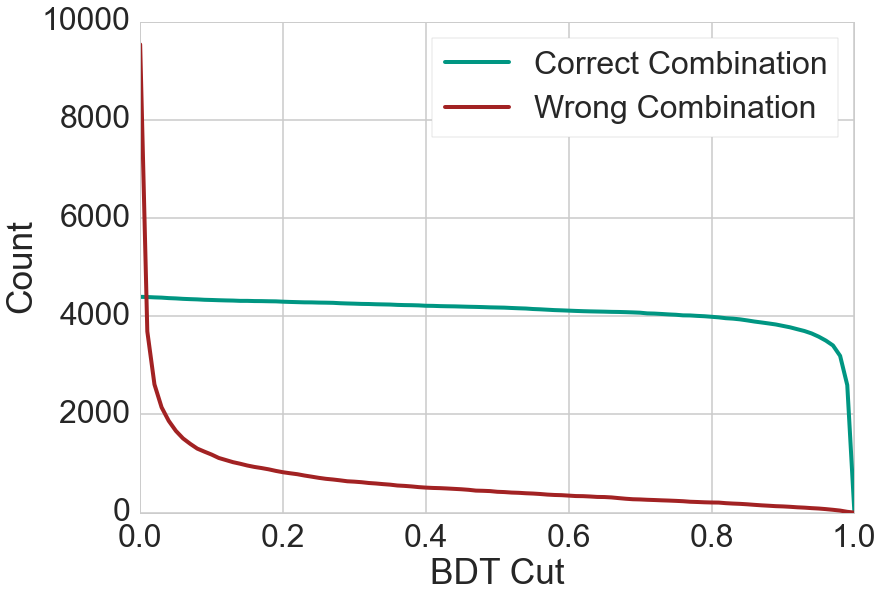
\includegraphics[width=0.7\linewidth]{figures/workflow/vxd_cdc_merger_count.png}
  \caption{Number of correct and wrong combinations passing the VXD--CDC-filter for different cut values. The number of wrong combinations can be reduced quite well with the filter.}
  \label{fig-vxd-cdc-count}  
  % Not comparable.
  % Final
\end{figure}

Presenting the results of the whole algorithm is complex, as there are many different subcases. First, only input tracks which are not classified as fakes by the MC track matcher algorithm are considered, because only then the decision if both the VXD and the CDC track belongs to the same MC particle can be made. The tracks are classified according to five subclasses:
\begin{zlist}
  \item The resulting track consists of both a VXD and a CDC track and both tracks are related to the same MC particle (correct).
  \item The resulting track consists of both a VXD and a CDC track, but they are related to different MC particles (wrong).
  \item The resulting track was not combined with a VXD track and also the related MC particle has no VXD hits (correct).
  \item The resulting track was not combined with a CDC track and also the related MC particle has no CDC hits (correct).
  \item The resulting track was not combined with a CDC track, but the related MC particle has CDC hits or it was not combined with a VXD track, but the related MC particle has VXD hits (also correct, but inefficient).
\end{zlist}

All resulting tracks from the module can be classified unambiguously into one of these categories. Table~\ref{tab-vxd-cdc-cases} shows the number of tracks in each category for different cuts on the BDT value. The number of correct and wrong combinations drops for tighter BDT cut values increasing the number of total resulting tracks (as more VXD or CDC tracks have no partner resulting in two instead of one track) and also the number of inefficient decisions (case 5). As expected, the number of tracks belonging in categories 3 and 4 is low, as the probability for a track to have no VXD or no CDC hits is low. As the presented module is planned to be installed in front of the fitting procedure with the already mentioned VXD--CDC-combiner after the fit, the number of not made combinations (case 5), is not that important.

\begin{table}
  \centering
  \caption{Number of tracks resulting from the VXD--CDC merger classified by the five categories as described in the text.}
  \hspace*{-0.55cm}
  \begin{tabular}{crlllll}
    \toprule
    BDT cut &  Total &         Case 1 &       Case 2 &       Case 3 &       Case 4 &         Case 5 \\
    \midrule
	0.0 &   9345 &  7361 (78.8 \%) &  643 (6.9 \%) &  215 (2.3 \%) &  327 (3.5 \%) &    799 (8.6 \%) \\
% 	0.1 &  10698 &  7712 (72.1 \%) &  298 (2.8 \%) &  612 (5.7 \%) &  390 (3.6 \%) &  1686 (15.8 \%) \\
% 	0.2 &  10855 &  7725 (71.2 \%) &  251 (2.3 \%) &  654 (6.0 \%) &  406 (3.7 \%) &  1819 (16.8 \%) \\
	0.3 &  10961 &  7723 (70.5 \%) &  227 (2.1 \%) &  698 (6.4 \%) &  417 (3.8 \%) &  1896 (17.3 \%) \\
% 	0.4 &  11041 &  7711 (69.8 \%) &  201 (1.8 \%) &  720 (6.5 \%) &  424 (3.8 \%) &  1985 (18.0 \%) \\
% 	0.5 &  11123 &  7708 (69.3 \%) &  176 (1.6 \%) &  748 (6.7 \%) &  427 (3.8 \%) &  2064 (18.6 \%) \\
	0.6 &  11211 &  7696 (68.6 \%) &  157 (1.4 \%) &  775 (6.9 \%) &  431 (3.8 \%) &  2152 (19.2 \%) \\
% 	0.7 &  11304 &  7672 (67.9 \%) &  143 (1.3 \%) &  797 (7.1 \%) &  436 (3.9 \%) &  2256 (20.0 \%) \\
% 	0.8 &  11452 &  7617 (66.5 \%) &  109 (1.0 \%) &  848 (7.4 \%) &  449 (3.9 \%) &  2429 (21.2 \%) \\
	0.9 &  11721 &  7490 (63.9 \%) &   68 (0.6 \%) &  921 (7.9 \%) &  460 (3.9 \%) &  2782 (23.7 \%) \\
    \bottomrule
  \end{tabular}
  \label{tab-vxd-cdc-cases}
  % Not comparable.
  % Final
\end{table}

For tracks which are marked as fakes by the MC matcher, these subclasses are undefined, as they need the matching information to a related MC particle. It is however possible to count the number of tracks, which were fakes before the combiner module and could be ``recovered'' by adding a CDC or VXD track. The ratio of these tracks to the full number of fakes (either CDC or VXD) are shown in figure~\ref{fig-vxd-cdc-recovered}. It can be seen that adding a VXD (or CDC) track to a fake track can turn it into a signal track because the number of correct hits is increased if the combination is correct. 

\begin{figure}
  \centering
  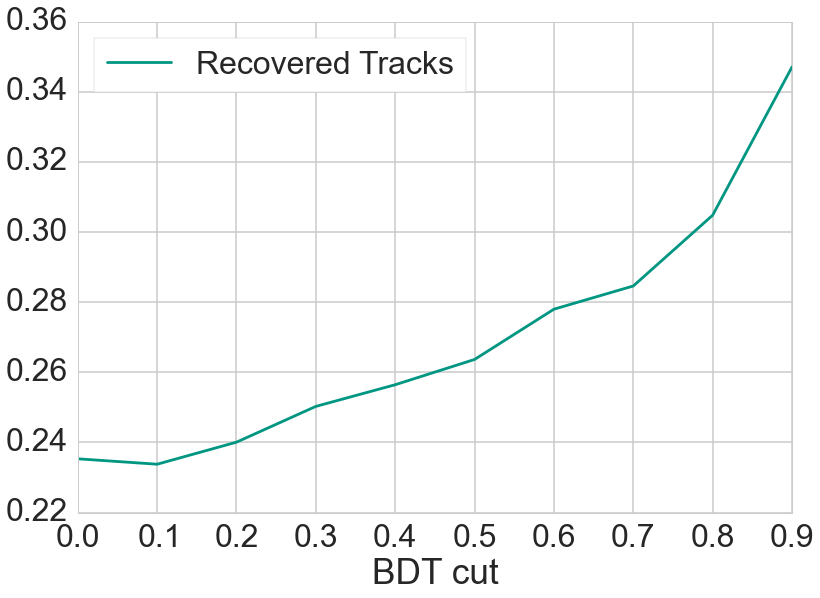
\includegraphics[width=0.7\linewidth]{figures/workflow/vxd_cdc_merger_recovered.png}
  \caption{Ratio of the resulting combinations that are no longer counted as fake to the full number of combinations, with one or both tracks marked as fake by the MC track matching algorithm.}
  \label{fig-vxd-cdc-recovered}
  % Not comparable.
  % Final
\end{figure}

Besides the already mentioned figures of merit for this particular algorithm, also the efficiencies and rates as for normal track finder algorithm can be calculated -- however, analyzing them is difficult. Table~\ref{tab-vxd-cdc-fom} shows the track finding figures of merit after the combiner module and for the track finders in the two detectors separately. For calculating the hit efficiencies, only the subdetectors are used where the tracks are defined -- so the figures of merit for the CDC track finders only use the CDC hits. A cut value of 0.8 is used. It can be seen, that the finding efficiency is much better than in the single subalgorithms, but one has to note that if a CDC track could not be matched to a VXD track, the track is still added to the result list and if it can be related to a MC particle, this particle still counts as found. As the same procedure is applied to the VXD tracks, the finding efficiencies of the CDC and VXD track finders ``add up''. This can be seen in the clone rate, which is higher in the combination than on the single tracking algorithms as some of the correct combinations were not made (cf.\ case 5 above). This however can be fixed by the subsequent combiner module after the track fit which is already implemented in the path. The hit efficiency drops when combining the detectors as it is now counted taken into account all hits (not only CDC or VXD separately) and the not-combined tracks decrease the efficiency as they have only hits in one detector. The fake rate and the number of wrong hits could also be reduced compared to the CDC track finder which indicates, that combining tracks can lead to recovering tracks as already discussed in figure~\ref{fig-vxd-cdc-recovered}.

\begin{table}
  \centering
  \caption{Track finders in the subdetectors on generic events without background and their combination in comparison.}
  \label{tab-vxd-cdc-fom}
  \begin{tabular}{lccc} \toprule
    & VXD & CDC & Both combined \\ \midrule
    Finding Efficiency   & 74.60 & 81.76 & 89.12 \\
    \quad on Primaries   & 94.20 & 85.30 & 95.33 \\ 
    Hit Efficiency       & 85.69 & 84.87 & 80.86 \\
    \quad on Primaries   & 86.72 & 90.77 & 86.95 \\ 
    Clone Rate           & 1.26 & 16.01 & 18.00 \\
    \quad on Primaries   & 1.32 & 7.41 & 12.07 \\ 
    Fake Rate            & 3.55 & 14.19 & 13.64 \\ 
    Wrong Hits per Track & 0.00 & 2.31 & 2.08 \\ \bottomrule
  \end{tabular}
  % Not comparable.
  % Final
\end{table}


% To define the purity of the algorithm, only the subset of tracks is considered, that have neither a fake as a CDC nor a VXD track. As for this condition a CDC as well as a VXD track must be present, all cases where the algorithm did not combine two tracks, are not taken into account here. Figure~\ref{fig-vxd-cdc-purity} shows the rate of correct matches and the purity. For defining these numbers, all made combinations by the module with a VXD and CDC track are used. A combination is tagged ``correct'' if the CDC and VXD track are both related to the same MC particle (as fakes are discarded in the initial condition, they both must be connected to a MC particle). The rate of correct matches shown in the figure is the number of correct combinations to the number of total combinations made by the module (so disregarding any efficiencies here). The purity is the number of non-fake tracks as tagged by the MC matching algorithm to the whole number of resulting tracks. The figure therefore leads to the conclusion, that for higher cut values over 97 \% of the tracks coming out of the module are correctly combined tracks. To deduce the efficiency of the algorithm

Further development to increase the separation power of the filter even more and to put the module into the full path of track finding and fitting has to be done, but these very preliminary results already show the great power of such an algorithm to increase the efficiency and also the computing performance. The reason for the latter is, that the combiner module after the track fit (as it is implemented in the moment) has to extrapolate the fitted CDC and VXD tracks through material to evaluate their tracking parameters on the same plane leading to a large number of material lookups needed before making the decision thus resulting in a large computing time.

